\documentclass[12pt]{article}
\usepackage[margin=1in]{geometry}
\usepackage{amsmath,amssymb,amsfonts}
\usepackage{graphicx}
\usepackage{booktabs}
\usepackage{setspace}
\usepackage{float}
\usepackage{caption}
\usepackage{hyperref}
\usepackage{xcolor}
\usepackage{subcaption}

\hypersetup{colorlinks=true,linkcolor=blue,citecolor=blue,urlcolor=blue}
\doublespacing

\title{\textbf{Estimating the Smets-Wouters Model with Different Observable Variables}}
\author{Dheeshana Koswatte\thanks{AI assistance (Grammarly) was used for grammar and language editing. All analysis, estimation, and intellectual content are the author's own work.}\\Department of Economics\\Texas Tech University}
\date{December 2025}

\begin{document}
\maketitle

\begin{abstract}
\noindent This paper estimates a variant of the Smets and Wouters (2007) DSGE model using different observable variables than those employed in the original study. Following the course assignment guidelines, the objective is to examine what the model reveals about the U.S. economy when estimated on non-standard macroeconomic indicators. The analysis attempts to replace all seven original observables; output growth, consumption growth, investment growth, hours worked, wage growth, inflation, and the federal funds rate; with unemployment, capacity utilization, credit spreads, stock returns, import price inflation, government spending growth, and the 10-year Treasury rate. The full specification fails to estimate as the Hessian matrix at the posterior mode is not positive definite, indicating fundamental identification problems. Diagnostic analysis reveals the structural source of this failure. Without direct observation of domestic inflation and wages, the Calvo price and wage stickiness parameters cannot be identified. A hybrid specification retaining four original observables while substituting three others succeeds, yielding converged MCMC chains and economically sensible posterior estimates. The Taylor rule coefficients differ notably from the original estimates, with a lower inflation response (1.65 versus 2.03) and higher shock persistence. These findings demonstrate that observable choice in DSGE estimation is constrained by model structure, not merely by statistical properties of the data.

\vspace{0.3cm}
\noindent\textbf{Keywords:} DSGE models, Bayesian estimation, identification, Smets-Wouters, observable variables

\noindent\textbf{JEL Classification:} C11, C32, E32, E52
\end{abstract}

\newpage
\tableofcontents
\newpage

%=============================================================================
\section{Introduction}
%=============================================================================

The Smets-Wouters (2007) model has become a benchmark for monetary policy analysis, demonstrating that medium-scale DSGE models estimated via Bayesian methods can compete with atheoretical vector autoregressions in forecasting while providing structural interpretation. Central banks worldwide employ variants of this framework for policy analysis.

This paper follows the ECO6361 course assignment to estimate an appropriate variant of the Smets-Wouters model using entirely different observed variables than those in the original study. The objective is to examine what the model tells us about the U.S. economy when disciplined by non-standard macroeconomic indicators. This exercise connects to a broader literature on the sensitivity of DSGE estimates to observable choice. Guerr\'{o}n-Quintana (2010) documented that changing observables can substantially alter structural parameter estimates. Canova, Ferroni, and Matthes (2014) examined observable selection in singular DSGE models. The identification literature, including Canova and Sala (2009) and Iskrev (2010), has highlighted that many DSGE parameters are only weakly identified by standard data.

The analysis proceeds in three stages, following a systematic approach to understanding identification constraints. First, an attempt is made to estimate the model using seven different observables: the unemployment rate, capacity utilization, credit spreads, stock market returns, import price inflation, government spending growth, and the 10-year Treasury rate. This specification fails as the Hessian matrix at the posterior mode is not positive definite, indicating fundamental identification problems.

Second, following Del Negro and Schorfheide (2008), who showed that prior specification can substantially affect identification in DSGE models, the priors are adjusted to better match the statistical properties of the proposed observables. This attempt also fails, with Dynare diagnostics identifying the Calvo price stickiness parameter ($\xi_p$) as unidentified. The repeated failure across different prior specifications suggests a \textit{structural} rather than \textit{statistical} problem.

Third, diagnostic analysis reveals why full substitution fails: without direct observation of domestic inflation and wages, the parameters governing nominal rigidities cannot be identified. A hybrid specification is then developed, retaining the original inflation, wage, consumption, and investment data while substituting capacity utilization for output, unemployment for hours, and the 10-year rate for the federal funds rate. This specification estimates successfully and yields economically interpretable results.

The main findings are threefold. First, full observable substitution in the Smets-Wouters framework is infeasible with the proposed variables due to structural identification constraints. Second, partial substitution succeeds when the retained observables correspond to model equations that require direct measurement. Third, the hybrid specification implies a more accommodative monetary policy rule and more persistent shocks than the original estimates, with implications for policy analysis.

The remainder of the paper is organized as follows. Section 2 describes the data. Section 3 presents the model specification, with particular attention to our modifications from Smets-Wouters (2007). Section 4 details the estimation methodology. Section 5 documents the estimation attempts and diagnostic analysis. Section 6 presents results from the successful hybrid specification. Section 7 discusses implications, and Section 8 concludes.

%=============================================================================
\section{Data}
%=============================================================================

\subsection{Sample Period and Sources}

All data cover the period 1967Q1--2004Q4, matching the original Smets and Wouters (2007) sample of 152 quarterly observations. This period encompasses several business cycles, including the recessions of 1969--70, 1973--75, 1980, 1981--82, 1990--91, and 2001. Data are obtained from the Federal Reserve Economic Data (FRED) database maintained by the Federal Reserve Bank of St. Louis.

\subsection{Original Smets-Wouters Observables}

The original estimation employs seven observables corresponding to the model's seven structural shocks:
\begin{enumerate}
    \item \textbf{Real GDP growth}: First difference of log real GDP per capita, measuring aggregate output dynamics
    \item \textbf{Real consumption growth}: First difference of log real personal consumption expenditures per capita
    \item \textbf{Real investment growth}: First difference of log real gross private domestic investment per capita
    \item \textbf{Hours worked}: Log hours worked per capita in the nonfarm business sector, demeaned
    \item \textbf{Real wage growth}: First difference of log real compensation per hour in the nonfarm business sector
    \item \textbf{Inflation}: First difference of log GDP deflator, measuring domestic price changes
    \item \textbf{Federal funds rate}: Quarterly average of the effective federal funds rate, the primary monetary policy instrument
\end{enumerate}

These series directly measure key objects in the model's structural equations. Output, consumption, and investment growth identify dynamics in the resource constraint and Euler equations. Hours worked identifies labor market clearing. Wage growth identifies the wage Phillips curve. Inflation identifies the price Phillips curve. The federal funds rate identifies the monetary policy rule.

\subsection{Proposed Different Observables}

Following the assignment guidelines, this paper proposes seven different observables intended to capture similar economic phenomena through alternative measurements:

\begin{enumerate}
    \item \textbf{Capacity utilization growth} (TCU): First difference of log capacity utilization index from the Federal Reserve Board. This measures the intensity of capital usage in manufacturing and is strongly procyclical, potentially serving as an alternative measure of output dynamics. Unlike GDP, which measures the level of production, capacity utilization measures how intensively existing capital is employed.
    
    \item \textbf{Negative unemployment rate} ($-$UNRATE): The civilian unemployment rate with sign reversed. By Okun's Law, unemployment moves inversely with economic activity and labor input. A higher unemployment rate corresponds to lower hours worked, so the sign reversal aligns the direction with the original hours observable.
    
    \item \textbf{Credit spread} (BAA $-$ GS10): The difference between Moody's Baa corporate bond yield and the 10-year Treasury yield. This spread captures default risk and financial conditions, potentially related to the model's risk premium shock. Credit spreads widen during recessions and financial stress, reflecting increased risk aversion.
    
    \item \textbf{Stock market returns} (S\&P 500): Quarterly returns on the S\&P 500 index. Stock prices are forward-looking and theoretically related to investment through Tobin's Q---firms invest when the market value of capital exceeds replacement cost.
    
    \item \textbf{Import price inflation} (IMPGSC1): Growth rate of the import price index for goods and services. As an alternative price measure, import inflation might discipline the model's nominal dynamics. However, import prices are determined by world markets and exchange rates rather than domestic price-setting behavior.
    
    \item \textbf{Government spending growth} (GCEC1): First difference of log real federal government consumption expenditures. This directly measures the exogenous government spending process in the model.
    
    \item \textbf{10-year Treasury rate} (GS10): The constant maturity 10-year Treasury yield. This long-term rate reflects expected future monetary policy and term premia, providing an alternative measure of monetary conditions to the federal funds rate.
\end{enumerate}

\subsection{Descriptive Statistics}

Table \ref{tab:stats} presents descriptive statistics for the proposed observables over the sample period.

\begin{table}[H]
\centering
\caption{Descriptive Statistics: Proposed Observable Variables}
\label{tab:stats}
\begin{tabular}{lccccc}
\toprule
Variable & Mean & Std. Dev. & Min & Max & AR(1) \\
\midrule
Capacity utilization growth & $-0.07$ & 1.89 & $-8.12$ & 5.94 & 0.31 \\
Unemployment rate & 6.04 & 1.50 & 3.40 & 10.67 & 0.98 \\
Credit spread (Baa$-$10yr) & 1.87 & 0.59 & 0.85 & 3.61 & 0.88 \\
Stock market returns & 1.87 & 6.03 & $-22.25$ & 18.80 & 0.27 \\
Import price inflation & 4.12 & 10.95 & $-16.16$ & 67.67 & 0.69 \\
Government spending growth & 0.62 & 0.88 & $-1.74$ & 2.66 & 0.07 \\
10-year Treasury rate & 7.62 & 2.41 & 3.64 & 14.86 & 0.97 \\
\bottomrule
\end{tabular}
\begin{flushleft}
\small \textit{Notes}: Sample: 1967Q1--2004Q4 (152 observations). All rates in percent per annum. Growth rates are quarterly percentage changes at annual rates. AR(1) is the first-order autocorrelation coefficient. Source: FRED.
\end{flushleft}
\end{table}

Several features merit attention. Persistence varies substantially across series: unemployment and the 10-year rate exhibit AR(1) coefficients near unity (0.98 and 0.97), indicating highly persistent processes that return slowly to their means. Government spending growth, by contrast, is nearly white noise with AR(1) of only 0.07, suggesting spending changes are largely unpredictable one quarter ahead. Credit spreads show intermediate persistence (0.88), widening during recessions and narrowing gradually during expansions.

Volatilities differ by an order of magnitude. Import price inflation is extremely volatile (standard deviation 10.95), driven by oil price shocks and exchange rate movements. Stock returns are also volatile (6.03), reflecting forward-looking asset price dynamics. Credit spreads are comparatively stable (0.59), as the spread between corporate and Treasury yields moves within a relatively narrow band except during financial crises.

The means reveal steady-state differences. The 10-year rate averaged 7.62\% over this period, substantially higher than recent experience. Unemployment averaged 6.04\%, and credit spreads averaged 1.87 percentage points.

\begin{figure}[H]
\centering
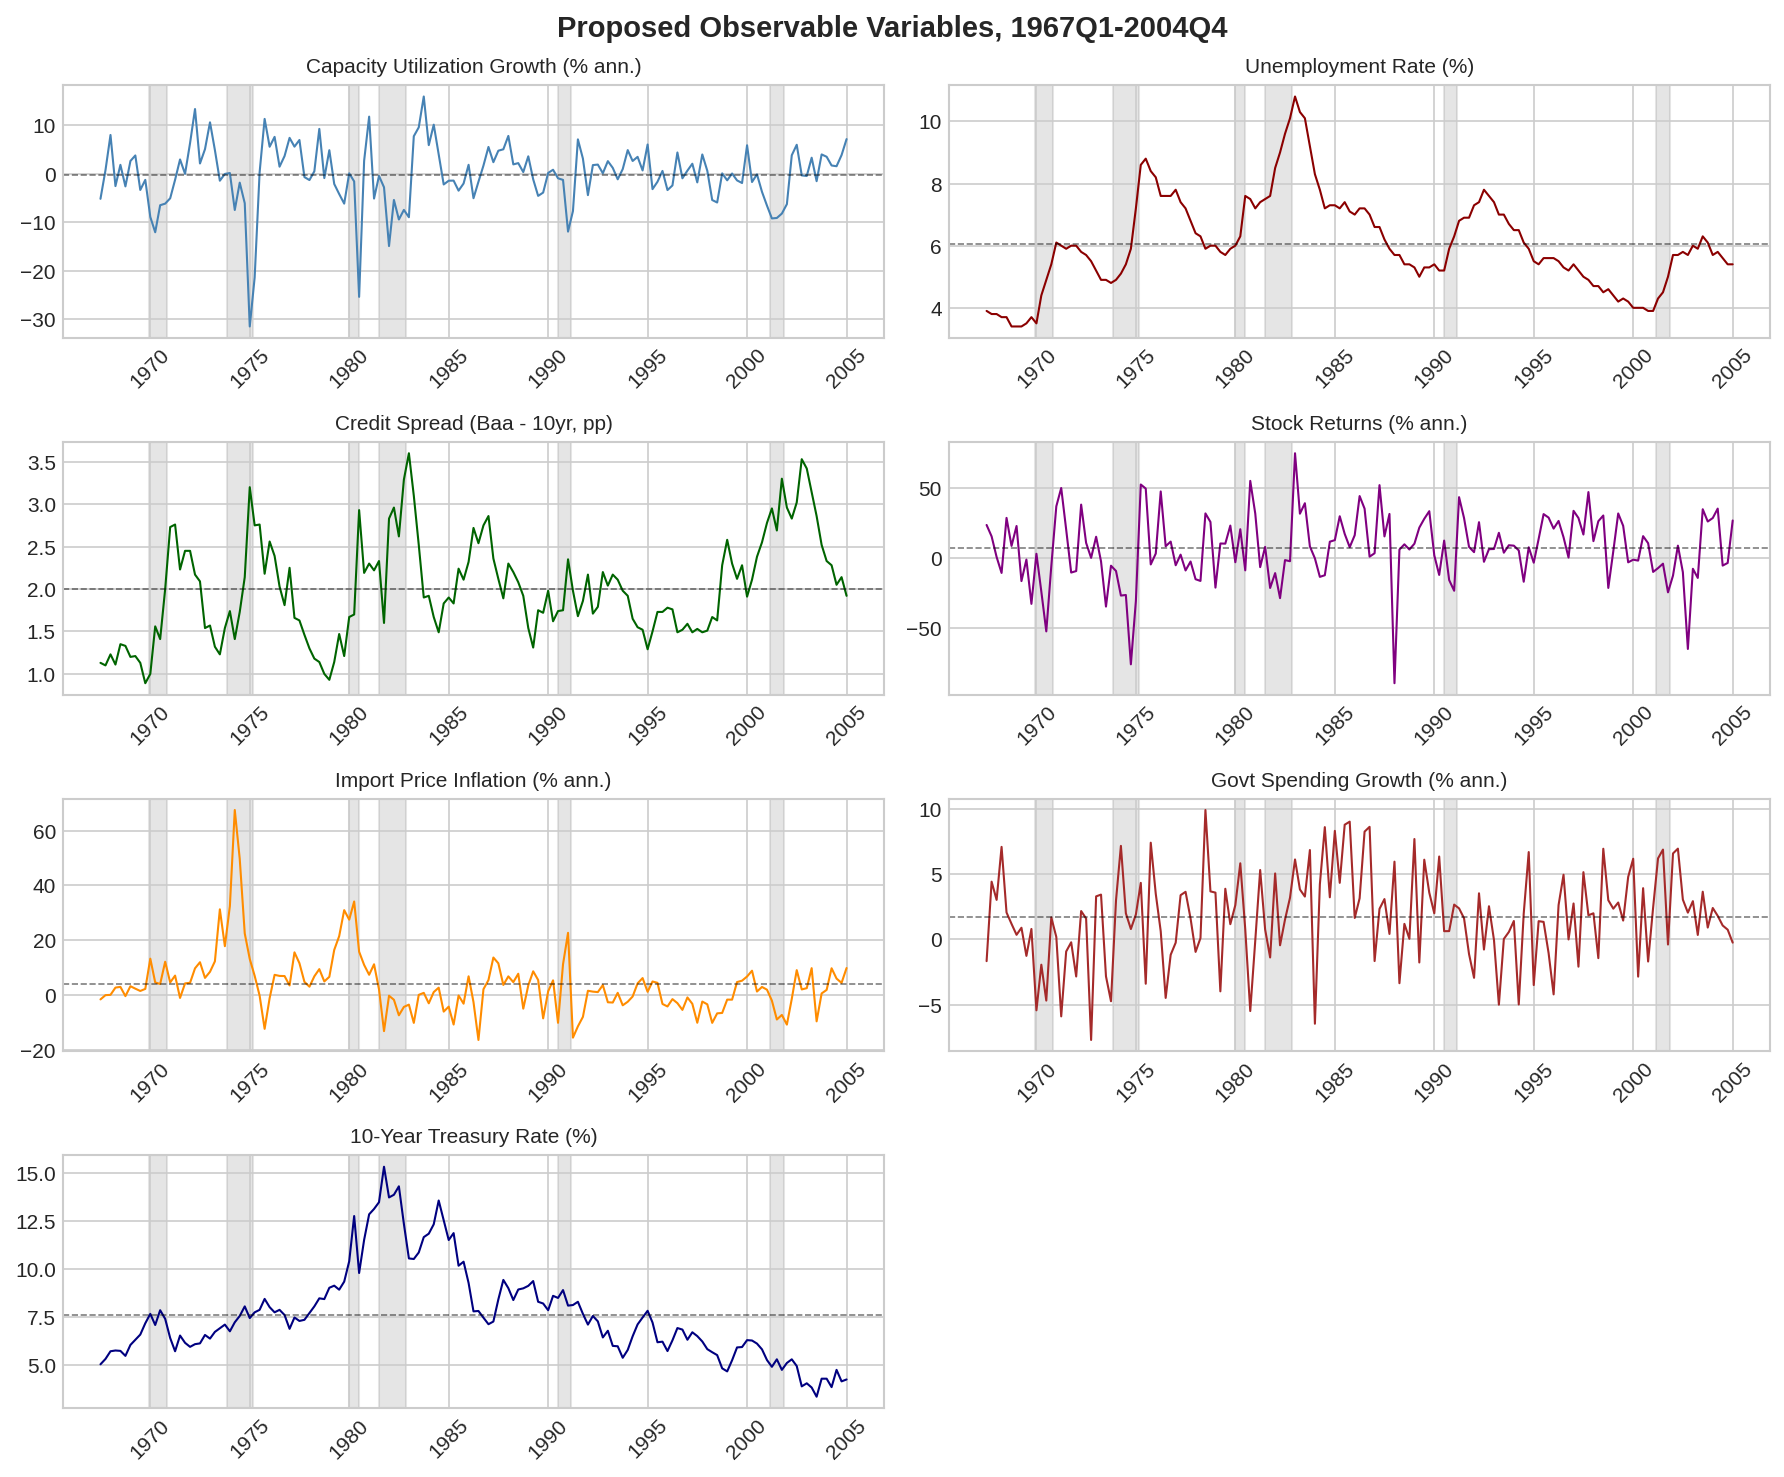
\includegraphics[width=0.95\textwidth]{figure1_alternative_observables.png}
\caption{Proposed Observable Variables, 1967Q1--2004Q4}
\label{fig:timeseries}
\end{figure}

Figure \ref{fig:timeseries} displays the time series with NBER recession dates shaded. The cyclical patterns are evident: unemployment rises sharply during recessions, capacity utilization falls, credit spreads widen, and stock returns decline. The 10-year rate shows a secular pattern, rising through the 1970s inflation, peaking in the early 1980s during the Volcker disinflation, and declining thereafter.

\subsection{Correlation with Original Observables}

A natural question is whether the proposed observables correlate with the original series they are intended to replace. Table \ref{tab:corr} reports these correlations.

\begin{table}[H]
\centering
\caption{Correlations: Proposed vs. Original Observables}
\label{tab:corr}
\begin{tabular}{llc}
\toprule
Proposed Observable & Original Observable & Correlation \\
\midrule
$-$Unemployment & Hours worked & 0.85 \\
10-year rate & Federal funds rate & 0.85 \\
Import price inflation & GDP deflator inflation & 0.37 \\
Capacity utilization growth & Output growth & 0.29 \\
Credit spread & Federal funds rate & 0.09 \\
Stock returns & Investment growth & $-0.10$ \\
Government spending growth & Output growth & $-0.03$ \\
\bottomrule
\end{tabular}
\begin{flushleft}
\small \textit{Notes}: Correlations computed over 1967Q1--2004Q4. Unemployment is sign-reversed for comparability with hours.
\end{flushleft}
\end{table}

The results are mixed. Two proposed observables correlate strongly with their targets: unemployment with hours ($-0.85$ when sign-adjusted) and the 10-year rate with the federal funds rate (0.85). These high correlations suggest these substitutions may succeed---both series measure the same underlying economic phenomena (labor market slack and monetary conditions) from different vantage points.

Three proposed observables show weak to moderate correlations: import inflation with domestic inflation (0.37), capacity utilization with output (0.29), and credit spreads with the policy rate (0.09). The weak correlation between credit spreads and the federal funds rate is particularly notable---these series measure fundamentally different aspects of financial markets.

Two proposed observables show essentially zero or negative correlation with their targets: stock returns with investment ($-0.10$) and government spending with output ($-0.03$). The negative correlation between stock returns and investment is counterintuitive given Tobin's Q theory, but reflects that stock prices are forward-looking while investment responds with lags.

\begin{figure}[H]
\centering
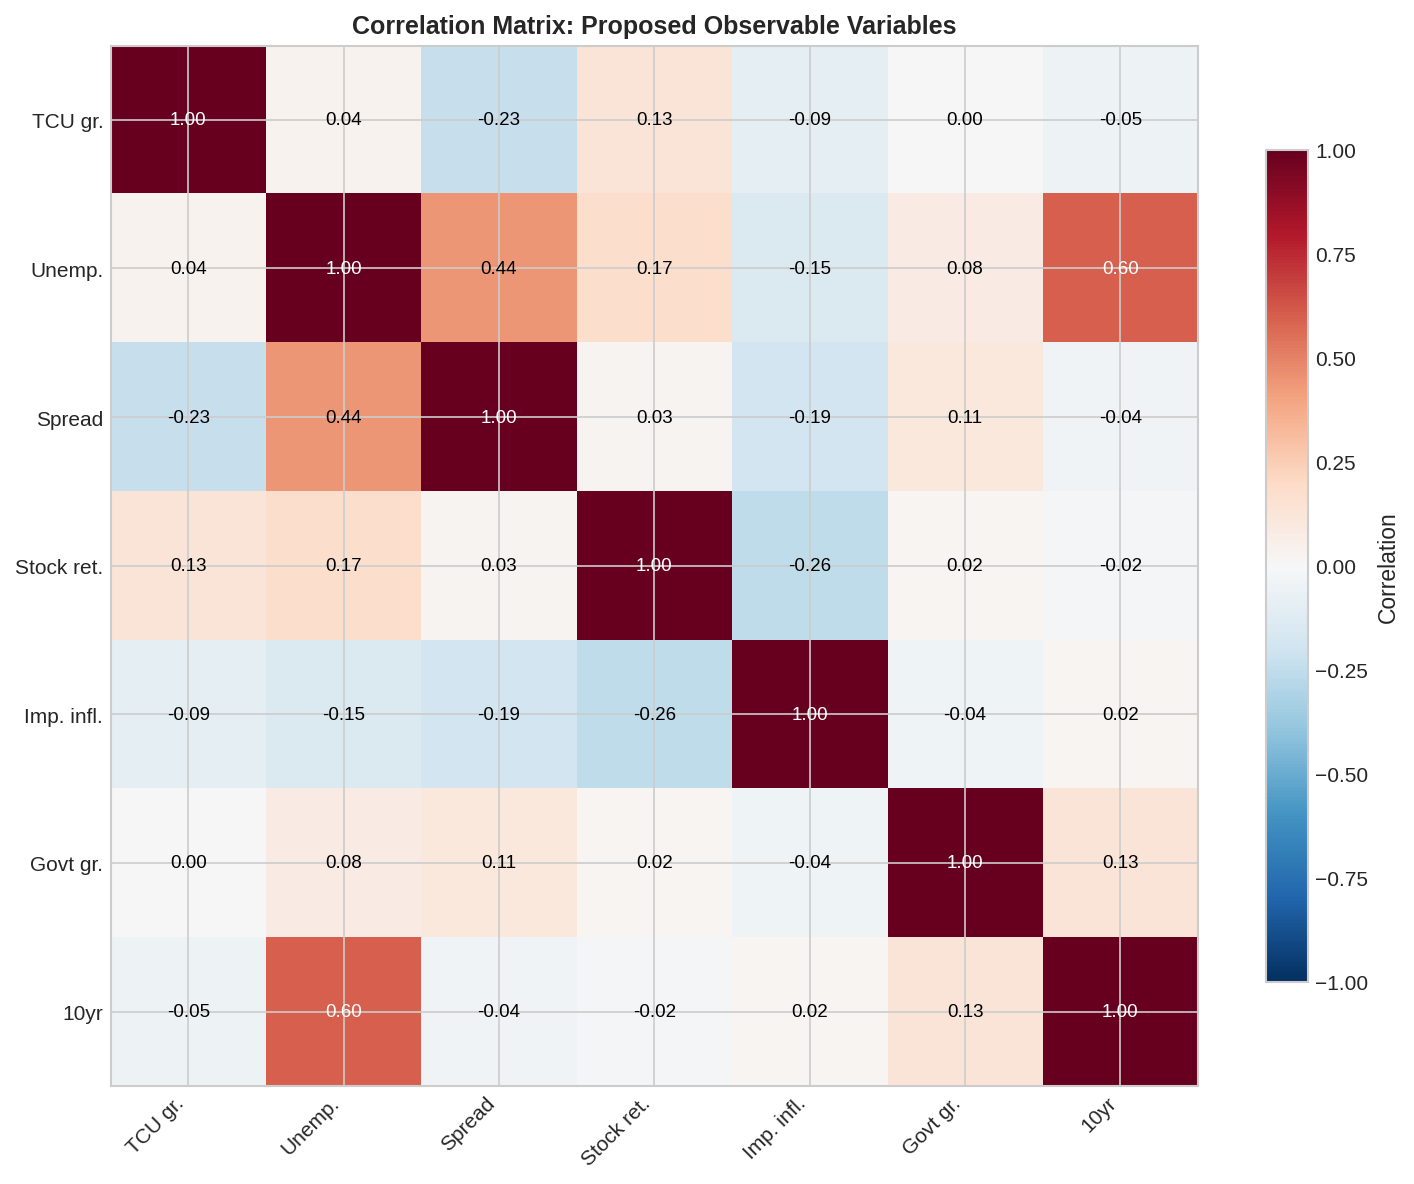
\includegraphics[width=0.9\textwidth]{figure2_correlation_matrix.png}
\caption{Correlation Structure: Proposed (left) vs. Original (right) Observables}
\label{fig:corrmatrix}
\end{figure}

Figure \ref{fig:corrmatrix} displays the full correlation matrices. The proposed observables show different internal correlation structure than the originals, which has implications for identification as discussed below.

A critical insight emerges from this analysis: \textit{correlation with the original observable is neither necessary nor sufficient for successful substitution}. As demonstrated in Section 5, capacity utilization (correlation 0.29 with output) substitutes successfully, while import inflation (correlation 0.37 with domestic inflation) does not. What matters is whether the proposed observable responds to the same structural forces as the original---a question of economic content, not statistical association.

%=============================================================================
\section{Model Specification}
%=============================================================================

This section presents the complete model specification. The structural equations follow Smets and Wouters (2007); the key modifications in this paper concern the measurement equations that link model variables to observables. Understanding this distinction is essential: the structural model remains unchanged, but the data used to estimate it differs.

\subsection{Overview of the Smets-Wouters Framework}

The Smets-Wouters model is a medium-scale New Keynesian DSGE model incorporating both nominal and real frictions. The model features:

\begin{itemize}
    \item \textbf{Households}: Infinitely-lived representative households with habit formation in consumption, supplying differentiated labor to unions that set wages subject to Calvo-style nominal rigidity with partial indexation to past inflation.
    
    \item \textbf{Firms}: Monopolistically competitive intermediate goods producers setting prices subject to Calvo-style nominal rigidity with partial indexation. Final goods are produced by competitive firms using a CES aggregator.
    
    \item \textbf{Capital}: Variable capital utilization and investment adjustment costs. Capital accumulates according to a standard law of motion with depreciation.
    
    \item \textbf{Government}: Exogenous government spending and a central bank following a Taylor-type interest rate rule.
    
    \item \textbf{Shocks}: Seven structural disturbances driving business cycle fluctuations.
\end{itemize}

\subsection{Notation and Definitions}

All model variables are expressed as log-deviations from steady state, denoted by lowercase letters. Key notation:

\begin{center}
\begin{tabular}{ll}
$y_t$ & Output \\
$c_t$ & Consumption \\
$i_t$ & Investment \\
$k_t$ & Capital services \\
$\bar{k}_t$ & Installed capital stock \\
$l_t$ & Hours worked \\
$w_t$ & Real wage \\
$r_t$ & Nominal interest rate \\
$\pi_t$ & Inflation \\
$q_t$ & Real value of capital (Tobin's Q) \\
$r^k_t$ & Rental rate of capital \\
$z_t$ & Capital utilization rate \\
$mc_t$ & Real marginal cost \\
\end{tabular}
\end{center}

Superscript $f$ denotes the flexible-price counterpart of a variable (e.g., $y^f_t$ is natural output). Steady-state values are denoted with bars (e.g., $\bar{y}$).

\subsection{Composite Parameters}

The model's reduced-form coefficients depend on combinations of deep parameters. The following composite parameters are derived from the deep structural parameters:

\textbf{Steady-state relationships:}
\begin{align}
\bar{\gamma} &= 1 + \frac{\gamma^*}{100} & \text{(gross trend growth rate)} \\
\bar{\beta} &= \frac{1}{1 + \bar{\beta}^*/100} & \text{(discount factor)} \\
\bar{\pi} &= 1 + \frac{\bar{\pi}^*}{100} & \text{(gross steady-state inflation)}
\end{align}

where $\gamma^*$, $\bar{\beta}^*$, and $\bar{\pi}^*$ are the net rates in percent (quarterly).

\textbf{Steady-state rental rate of capital:}
\begin{equation}
\bar{r}^k = \bar{\beta}^{-1}\bar{\gamma}^{\sigma_c} - (1-\delta)
\end{equation}

This expression comes from the steady-state Euler equation for capital, equating the return on capital to the household's discount rate adjusted for trend growth and risk aversion.

\textbf{Steady-state real wage:}
\begin{equation}
\bar{w} = \left(\frac{\alpha^\alpha(1-\alpha)^{1-\alpha}}{\phi_p \cdot (\bar{r}^k)^\alpha}\right)^{\frac{1}{1-\alpha}}
\end{equation}

\textbf{Great ratios:}
\begin{align}
\frac{\bar{k}}{\bar{y}} &= \phi_p\left(\frac{\bar{k}}{\bar{l}}\right)^{\alpha-1} \\
\frac{\bar{i}}{\bar{y}} &= \left(1-\frac{1-\delta}{\bar{\gamma}}\right)\frac{\bar{k}}{\bar{y}} \\
\frac{\bar{c}}{\bar{y}} &= 1 - \bar{g} - \frac{\bar{i}}{\bar{y}}
\end{align}

where $\bar{g}$ is the steady-state government spending share of output.

\subsection{Household Sector}

\subsubsection{Consumption Euler Equation}

The consumption Euler equation with external habit formation (parameter $h$) is:
\begin{equation}
\boxed{c_t = \frac{h/\bar{\gamma}}{1+h/\bar{\gamma}}c_{t-1} + \frac{1}{1+h/\bar{\gamma}}\mathbb{E}_t c_{t+1} - \frac{1-h/\bar{\gamma}}{\sigma_c(1+h/\bar{\gamma})}(r_t - \mathbb{E}_t\pi_{t+1}) + \frac{1-h/\bar{\gamma}}{\sigma_c(1+h/\bar{\gamma})}\varepsilon^b_t}
\label{eq:euler}
\end{equation}

This equation embodies the household's intertemporal optimization. Current consumption depends on:
\begin{itemize}
    \item \textit{Past consumption} ($c_{t-1}$): Due to habit formation, households derive utility from consumption relative to a habit stock. Higher $h$ means stronger dependence on past consumption.
    \item \textit{Expected future consumption} ($\mathbb{E}_t c_{t+1}$): Standard consumption smoothing motive.
    \item \textit{Real interest rate} ($r_t - \mathbb{E}_t\pi_{t+1}$): Higher real rates induce substitution toward future consumption.
    \item \textit{Risk premium shock} ($\varepsilon^b_t$): A preference disturbance affecting the marginal utility of consumption.
\end{itemize}

\textbf{Key parameters}: $\sigma_c$ (coefficient of relative risk aversion), $h$ (habit formation)

\textbf{Identifying observable}: Consumption growth is required to identify these parameters. The dynamics of consumption relative to interest rates and its own lags pin down $\sigma_c$ and $h$.

\subsubsection{Labor Supply}

The intratemporal condition equating the marginal rate of substitution to the real wage:
\begin{equation}
\boxed{w_t = \sigma_l l_t + \frac{1}{1-h/\bar{\gamma}}c_t - \frac{h/\bar{\gamma}}{1-h/\bar{\gamma}}c_{t-1}}
\label{eq:laborsupply}
\end{equation}

The real wage equals the marginal disutility of labor (scaled by $\sigma_l$) plus the marginal utility of consumption (affected by habit).

\textbf{Key parameter}: $\sigma_l$ (inverse Frisch elasticity of labor supply)

\subsection{Wage Setting}

Wages are set by monopolistically competitive labor unions facing Calvo-style nominal rigidity. With probability $\xi_w$, a union cannot re-optimize and instead indexes wages to past inflation (with weight $\iota_w$) and trend productivity growth.

The wage Phillips curve is:
\begin{equation}
\boxed{\begin{aligned}
w_t = &\frac{1}{1+\bar{\beta}\bar{\gamma}}w_{t-1} + \frac{\bar{\beta}\bar{\gamma}}{1+\bar{\beta}\bar{\gamma}}\mathbb{E}_t w_{t+1} + \frac{\iota_w}{1+\bar{\beta}\bar{\gamma}}\pi_{t-1} \\
&- \frac{1+\bar{\beta}\bar{\gamma}\iota_w}{1+\bar{\beta}\bar{\gamma}}\pi_t + \frac{\bar{\beta}\bar{\gamma}}{1+\bar{\beta}\bar{\gamma}}\mathbb{E}_t\pi_{t+1} \\
&+ \frac{(1-\xi_w)(1-\bar{\beta}\bar{\gamma}\xi_w)}{(1+\bar{\beta}\bar{\gamma})\xi_w[(\phi_w-1)\varepsilon_w+1]}(w^*_t - w_t) + \varepsilon^w_t
\end{aligned}}
\label{eq:wage}
\end{equation}

where $w^*_t$ is the desired wage (from labor supply) and $\varepsilon^w_t$ is a wage markup shock.

\textbf{Key parameters}: $\xi_w$ (Calvo wage stickiness---probability of not re-optimizing), $\iota_w$ (wage indexation to past inflation)

\textbf{Identifying observable}: Wage growth is required. The parameter $\xi_w$ determines how quickly wages adjust to desired levels; without observing wage dynamics, this speed of adjustment cannot be identified.

\subsection{Production Sector}

\subsubsection{Production Function}

Output is produced using capital services and labor with a Cobb-Douglas technology:
\begin{equation}
\boxed{y_t = \phi_p[\alpha k_t + (1-\alpha)l_t + \varepsilon^a_t]}
\label{eq:production}
\end{equation}

where $\alpha$ is the capital share, $\phi_p$ is the steady-state price markup (related to fixed costs), and $\varepsilon^a_t$ is total factor productivity.

\textbf{Key parameter}: $\alpha$ (capital share, typically calibrated to 0.24 based on labor's share of income)

\subsubsection{Marginal Cost}

Real marginal cost is the ratio of factor prices to marginal products:
\begin{equation}
\boxed{mc_t = \alpha r^k_t + (1-\alpha)w_t - \varepsilon^a_t}
\label{eq:mc}
\end{equation}

Higher rental rates or wages raise marginal cost; higher productivity reduces it.

\subsubsection{Capital Services}

Capital services combine the installed capital stock with the utilization rate:
\begin{equation}
\boxed{k_t = \bar{k}_{t-1} + z_t}
\label{eq:capitalservices}
\end{equation}

Firms can vary capital input in the short run by adjusting utilization intensity.

\subsubsection{Capital Utilization}

The utilization rate responds to the rental rate of capital:
\begin{equation}
\boxed{z_t = \frac{1-\psi}{\psi}r^k_t}
\label{eq:utilization}
\end{equation}

where $\psi \in (0,1)$ governs the elasticity of utilization with respect to the rental rate. Higher rental rates induce more intensive capital use, but this accelerates depreciation.

\textbf{Key parameter}: $\psi$ (utilization cost elasticity)

\subsubsection{Rental Rate of Capital}

In equilibrium, the rental rate equals the marginal product of capital:
\begin{equation}
\boxed{r^k_t = w_t + l_t - k_t}
\label{eq:rental}
\end{equation}

This comes from cost minimization by firms.

\subsection{Price Setting: The Phillips Curve}

\textbf{This equation is central to understanding the identification failure.}

Prices are set by monopolistically competitive firms facing Calvo-style nominal rigidity. With probability $\xi_p$, a firm cannot re-optimize its price and instead indexes to past inflation with weight $\iota_p$.

The price Phillips curve is:
\begin{equation}
\boxed{\pi_t = \frac{\iota_p}{1+\bar{\beta}\bar{\gamma}\iota_p}\pi_{t-1} + \frac{\bar{\beta}\bar{\gamma}}{1+\bar{\beta}\bar{\gamma}\iota_p}\mathbb{E}_t\pi_{t+1} + \kappa_p \cdot mc_t + \varepsilon^p_t}
\label{eq:phillips}
\end{equation}

where the slope coefficient is:
\begin{equation}
\kappa_p = \frac{(1-\xi_p)(1-\bar{\beta}\bar{\gamma}\xi_p)}{\xi_p[(\phi_p-1)\varepsilon_p+1](1+\bar{\beta}\bar{\gamma}\iota_p)}
\label{eq:kappa}
\end{equation}

\textbf{Key parameters}: $\xi_p$ (Calvo price stickiness), $\iota_p$ (price indexation)

\textbf{Why domestic inflation is required for identification}: The Calvo parameter $\xi_p$ appears only in the slope coefficient $\kappa_p$. To identify $\xi_p$, the econometrician must observe how inflation responds to marginal cost movements. Specifically:
\begin{itemize}
    \item A lower $\xi_p$ (more flexible prices) implies a steeper Phillips curve---inflation responds more strongly to marginal cost.
    \item A higher $\xi_p$ (stickier prices) implies a flatter Phillips curve---inflation is less responsive.
\end{itemize}

\textbf{Why import price inflation fails}: Import prices are determined by:
\begin{enumerate}
    \item World commodity prices (especially oil)
    \item Exchange rate movements
    \item Foreign production costs
\end{enumerate}

None of these factors relate to domestic firms' price-setting frequency. Import inflation with correlation 0.37 to domestic inflation does not identify $\xi_p$ because it responds to different economic forces. The Phillips curve describes \textit{domestic} price-setting behavior; import prices are determined abroad.

\subsection{Investment}

Investment dynamics with adjustment costs:
\begin{equation}
\boxed{i_t = \frac{1}{1+\bar{\beta}\bar{\gamma}}i_{t-1} + \frac{\bar{\beta}\bar{\gamma}}{1+\bar{\beta}\bar{\gamma}}\mathbb{E}_t i_{t+1} + \frac{1}{\bar{\gamma}^2\varphi(1+\bar{\beta}\bar{\gamma})}q_t + \varepsilon^i_t}
\label{eq:investment}
\end{equation}

Investment exhibits inertia due to adjustment costs (parameter $\varphi$). Higher Tobin's Q stimulates investment; the investment-specific technology shock $\varepsilon^i_t$ shifts the efficiency of transforming consumption goods into capital.

\textbf{Key parameter}: $\varphi$ (investment adjustment cost)

\textbf{Identifying observable}: Investment growth is required. The parameter $\varphi$ determines how quickly investment responds to changes in Q; observing investment dynamics pins down this speed of adjustment.

\subsection{Tobin's Q}

The real value of capital evolves as:
\begin{equation}
\boxed{q_t = -(r_t - \mathbb{E}_t\pi_{t+1}) + \frac{1-\delta}{\bar{r}^k+1-\delta}\mathbb{E}_t q_{t+1} + \frac{\bar{r}^k}{\bar{r}^k+1-\delta}\mathbb{E}_t r^k_{t+1} + \tilde{\varepsilon}^b_t}
\label{eq:tobin}
\end{equation}

This is an asset pricing equation. Q falls when real interest rates rise (discounting effect) and rises with expected future Q and rental rates. The term $\tilde{\varepsilon}^b_t$ captures risk premium effects on asset valuation.

\subsection{Capital Accumulation}

The law of motion for the installed capital stock:
\begin{equation}
\boxed{\bar{k}_t = \frac{1-\delta}{\bar{\gamma}}\bar{k}_{t-1} + \left(1-\frac{1-\delta}{\bar{\gamma}}\right)i_t + \left(1-\frac{1-\delta}{\bar{\gamma}}\right)\bar{\gamma}^2\varphi\varepsilon^i_t}
\label{eq:capital}
\end{equation}

Capital depreciates at rate $\delta$ and is augmented by investment. The investment-specific shock affects the efficiency of capital formation.

\subsection{Aggregate Resource Constraint}

Market clearing requires:
\begin{equation}
\boxed{y_t = \frac{\bar{c}}{\bar{y}}c_t + \frac{\bar{i}}{\bar{y}}i_t + \frac{\bar{r}^k\bar{k}}{\bar{y}}z_t + \varepsilon^g_t}
\label{eq:resource}
\end{equation}

Output is absorbed by consumption, investment, capital utilization costs, and government spending. The shock $\varepsilon^g_t$ captures both government spending and net exports.

\subsection{Monetary Policy Rule}

The central bank follows a Taylor-type interest rate rule:
\begin{equation}
\boxed{r_t = \rho r_{t-1} + (1-\rho)[r_\pi\pi_t + r_y(y_t - y^f_t)] + r_{\Delta y}[(y_t - y^f_t) - (y_{t-1} - y^f_{t-1})] + \varepsilon^r_t}
\label{eq:taylor}
\end{equation}

The policy rate responds to:
\begin{itemize}
    \item \textit{Lagged interest rate} ($r_{t-1}$): Interest rate smoothing with coefficient $\rho$
    \item \textit{Inflation} ($\pi_t$): With coefficient $r_\pi$, typically exceeding 1 for determinacy
    \item \textit{Output gap} ($y_t - y^f_t$): With coefficient $r_y$
    \item \textit{Output gap growth} ($\Delta(y_t - y^f_t)$): With coefficient $r_{\Delta y}$
    \item \textit{Monetary policy shock} ($\varepsilon^r_t$): Unexpected policy deviations
\end{itemize}

\textbf{Key parameters}: $\rho$ (smoothing), $r_\pi$ (inflation response), $r_y$ (output gap response), $r_{\Delta y}$ (output growth response)

\textbf{Identifying observable}: An interest rate measure is required. The coefficients describe how the policy instrument responds to economic conditions.

\subsection{Shock Processes}

The model features seven structural shocks, each following an AR(1) process:
\begin{align}
\varepsilon^a_t &= \rho_a \varepsilon^a_{t-1} + \eta^a_t & \text{(Total factor productivity)} \label{eq:shock_a}\\
\varepsilon^b_t &= \rho_b \varepsilon^b_{t-1} + \eta^b_t & \text{(Risk premium / preference)} \label{eq:shock_b}\\
\varepsilon^g_t &= \rho_g \varepsilon^g_{t-1} + \eta^g_t + \rho_{ga}\eta^a_t & \text{(Government spending)} \label{eq:shock_g}\\
\varepsilon^i_t &= \rho_i \varepsilon^i_{t-1} + \eta^i_t & \text{(Investment-specific technology)} \label{eq:shock_i}\\
\varepsilon^r_t &= \rho_r \varepsilon^r_{t-1} + \eta^r_t & \text{(Monetary policy)} \label{eq:shock_r}\\
\varepsilon^p_t &= \rho_p \varepsilon^p_{t-1} + \eta^p_t - \mu_p\eta^p_{t-1} & \text{(Price markup)} \label{eq:shock_p}\\
\varepsilon^w_t &= \rho_w \varepsilon^w_{t-1} + \eta^w_t - \mu_w\eta^w_{t-1} & \text{(Wage markup)} \label{eq:shock_w}
\end{align}

where $\eta^j_t \sim N(0, \sigma^2_j)$ are i.i.d. innovations.

Special features:
\begin{itemize}
    \item The government spending shock includes a spillover from productivity ($\rho_{ga}$), capturing that government spending may respond to economic conditions.
    \item The markup shocks include MA(1) components ($\mu_p$, $\mu_w$), allowing for more flexible short-run dynamics.
\end{itemize}

\subsection{Flexible-Price Economy}

The model also computes a ``natural'' or flexible-price equilibrium by setting $\xi_p = \xi_w = 0$. This yields natural output $y^f_t$ and the natural interest rate $r^f_t$, which enter the policy rule as benchmarks. The output gap $(y_t - y^f_t)$ measures the deviation of actual output from its flexible-price counterpart.

\subsection{Measurement Equations: Our Modification}

The measurement equations link the model's state variables to observable data. \textbf{This is where our specification differs from Smets and Wouters (2007).}

\subsubsection{Original SW(2007) Measurement Equations}

Smets and Wouters use seven measurement equations linking model variables to their seven observables:
\begin{align}
\Delta\log Y_t^{obs} &= \bar{\gamma} + y_t - y_{t-1} \label{eq:meas_y_orig}\\
\Delta\log C_t^{obs} &= \bar{\gamma} + c_t - c_{t-1} \label{eq:meas_c_orig}\\
\Delta\log I_t^{obs} &= \bar{\gamma} + i_t - i_{t-1} \label{eq:meas_i_orig}\\
\log L_t^{obs} &= \bar{l} + l_t \label{eq:meas_l_orig}\\
\Delta\log W_t^{obs} &= \bar{\gamma} + w_t - w_{t-1} \label{eq:meas_w_orig}\\
\pi_t^{obs} &= \bar{\pi} + \pi_t \label{eq:meas_pi_orig}\\
R_t^{obs} &= \bar{r} + r_t \label{eq:meas_r_orig}
\end{align}

The constants $\bar{\gamma}$, $\bar{l}$, $\bar{\pi}$, $\bar{r}$ represent steady-state values, allowing the model (expressed in deviations) to match data with non-zero means.

\subsubsection{Hybrid Model Measurement Equations}

Our hybrid specification modifies three measurement equations while retaining four from the original:

\textbf{Modified measurement equations (3 different observables):}
\begin{align}
\Delta\log TCU_t^{obs} &= \bar{\gamma}_{tcu} + y_t - y_{t-1} & \text{(Capacity util. for output)} \label{eq:meas_tcu}\\
-UNRATE_t^{obs} &= \bar{l} + l_t & \text{(Unemployment for hours)} \label{eq:meas_unemp}\\
GS10_t^{obs}/4 &= \bar{r}_{10y} + r_t & \text{(10-year rate for fed funds)} \label{eq:meas_10y}
\end{align}

\textbf{Retained original measurement equations (4 original observables):}
\begin{align}
\Delta\log C_t^{obs} &= \bar{\gamma} + c_t - c_{t-1} & \text{(Consumption)} \label{eq:meas_c_hybrid}\\
\Delta\log I_t^{obs} &= \bar{\gamma} + i_t - i_{t-1} & \text{(Investment)} \label{eq:meas_i_hybrid}\\
\Delta\log W_t^{obs} &= \bar{\gamma} + w_t - w_{t-1} & \text{(Wages)} \label{eq:meas_w_hybrid}\\
\pi_t^{obs} &= \bar{\pi} + \pi_t & \text{(Inflation)} \label{eq:meas_pi_hybrid}
\end{align}

\subsubsection{Rationale for Retained Observables}

Each retained observable is necessary for identifying specific structural parameters:

\begin{itemize}
    \item \textbf{Inflation} (equation \ref{eq:meas_pi_hybrid}): Required to identify $\xi_p$ and $\iota_p$ in the Phillips curve. Without observing domestic inflation dynamics, the frequency and indexation of price adjustment cannot be inferred.
    
    \item \textbf{Wages} (equation \ref{eq:meas_w_hybrid}): Required to identify $\xi_w$ and $\iota_w$ in the wage equation. Wage dynamics reveal how quickly wages adjust to desired levels.
    
    \item \textbf{Consumption} (equation \ref{eq:meas_c_hybrid}): Required to identify $h$ and $\sigma_c$ in the Euler equation. The persistence and interest-sensitivity of consumption pin down habit formation and risk aversion.
    
    \item \textbf{Investment} (equation \ref{eq:meas_i_hybrid}): Required to identify $\varphi$ in the investment equation. Investment dynamics reveal the magnitude of adjustment costs.
\end{itemize}

\subsubsection{Rationale for Substituted Observables}

The three substituted observables measure the same economic concepts as the originals:

\begin{itemize}
    \item \textbf{Capacity utilization for output} (equation \ref{eq:meas_tcu}): Both measure cyclical economic conditions. Capacity utilization rises and falls with the business cycle, just as output growth does. The key is that both respond to the same underlying demand and supply shocks in the model.
    
    \item \textbf{Unemployment for hours} (equation \ref{eq:meas_unemp}): Both measure labor market slack. By Okun's Law, unemployment and hours are strongly negatively correlated ($\rho = -0.85$). When firms reduce labor input (lower hours), unemployment rises.
    
    \item \textbf{10-year rate for federal funds} (equation \ref{eq:meas_10y}): Both measure monetary conditions. The 10-year rate reflects expected future policy and thus contains information about the systematic component of monetary policy, even if it is less directly controlled by the Fed.
\end{itemize}

\subsection{Steady-State Constants}

The measurement equation constants are calibrated to sample means:
\begin{align*}
\bar{\gamma}_{tcu} &= -0.0686 & \text{(Capacity utilization growth mean)} \\
\bar{\gamma} &= 0.4857 & \text{(Consumption/investment growth mean)} \\
\bar{\gamma}_w &= 0.3997 & \text{(Wage growth mean)} \\
\bar{l} &= 0.0 & \text{(Demeaned unemployment)} \\
\bar{\pi} &= 1.0165 & \text{(Inflation mean, quarterly \%)} \\
\bar{r}_{10y} &= 1.9058 & \text{(10-year rate mean, quarterly)}
\end{align*}

\subsection{Summary: Equations, Parameters, and Identification}

Table \ref{tab:equations} summarizes the model equations, key parameters, and identifying observables.

\begin{table}[H]
\centering
\caption{Model Equations, Parameters, and Identifying Observables}
\label{tab:equations}
\small
\begin{tabular}{llll}
\toprule
Equation & Key Parameters & Identifying Observable & Status \\
\midrule
Euler (eq. \ref{eq:euler}) & $\sigma_c$, $h$ & Consumption & Retained \\
Labor supply (eq. \ref{eq:laborsupply}) & $\sigma_l$ & Hours/Unemployment & Substituted \\
Wage Phillips (eq. \ref{eq:wage}) & $\xi_w$, $\iota_w$ & Wages & Retained \\
Price Phillips (eq. \ref{eq:phillips}) & $\xi_p$, $\iota_p$ & \textbf{Domestic inflation} & Retained \\
Investment (eq. \ref{eq:investment}) & $\varphi$ & Investment & Retained \\
Taylor rule (eq. \ref{eq:taylor}) & $\rho$, $r_\pi$, $r_y$, $r_{\Delta y}$ & Interest rate & Substituted \\
Resource (eq. \ref{eq:resource}) & --- & Output/Cap. util. & Substituted \\
Shocks (eq. \ref{eq:shock_a}--\ref{eq:shock_w}) & $\rho_j$, $\sigma_j$ & All observables & --- \\
\bottomrule
\end{tabular}
\end{table}

The critical insight is that the Price Phillips Curve (equation \ref{eq:phillips}) requires domestic inflation for identification. This is not merely a suggestion---it is a mathematical constraint. The Calvo parameter $\xi_p$ appears only through the slope $\kappa_p$, and estimating this slope requires observing how domestic prices respond to marginal costs. No alternative observable can substitute for this without modifying the model structure itself.


%=============================================================================
\section{Estimation Methodology}
%=============================================================================

\subsection{Bayesian Estimation Framework}

The model is estimated using Bayesian methods, which combine prior information about parameters with the likelihood of the data. The posterior distribution is:
\begin{equation}
p(\theta|Y^T) \propto p(Y^T|\theta) \cdot p(\theta)
\end{equation}

where $\theta$ is the vector of structural parameters, $Y^T = \{y_1, \ldots, y_T\}$ denotes the observed data, $p(Y^T|\theta)$ is the likelihood function, and $p(\theta)$ is the prior distribution.

The likelihood is computed using the Kalman filter. The linearized model can be written in state-space form:
\begin{align}
s_t &= A(\theta)s_{t-1} + B(\theta)\varepsilon_t & \text{(State equation)} \\
y_t &= C(\theta)s_t + D(\theta) & \text{(Measurement equation)}
\end{align}

where $s_t$ is the state vector, $\varepsilon_t$ are the structural shocks, and $y_t$ are the observables. The Kalman filter recursively computes the likelihood by predicting each observation given past data and updating the state estimate.

\subsection{Prior Distributions}

Prior distributions are specified following Smets and Wouters (2007), with some modifications for the proposed observables. Table \ref{tab:priors} reports the prior distributions.

\begin{table}[H]
\centering
\caption{Prior Distributions}
\label{tab:priors}
\scriptsize
\setlength{\tabcolsep}{3pt}
\renewcommand{\arraystretch}{0.85}
\begin{tabular}{@{}llccc@{}}
\toprule
Parameter & Description & Distribution & Mean & Std. Dev. \\
\midrule
\multicolumn{5}{l}{\textit{Structural Parameters}} \\
$\sigma_c$ & Risk aversion & Normal & 1.50 & 0.375 \\
$\sigma_l$ & Inverse Frisch elasticity & Normal & 2.00 & 0.75 \\
$h$ & Habit formation & Beta & 0.70 & 0.10 \\
$\xi_w$ & Calvo wages & Beta & 0.50 & 0.10 \\
$\xi_p$ & Calvo prices & Beta & 0.50 & 0.10 \\
$\iota_w$ & Wage indexation & Beta & 0.50 & 0.15 \\
$\iota_p$ & Price indexation & Beta & 0.50 & 0.15 \\
$\psi$ & Capital utilization & Beta & 0.50 & 0.15 \\
$\varphi$ & Investment adjustment cost & Normal & 4.00 & 1.50 \\
$\phi_p$ & Fixed cost share & Normal & 1.25 & 0.125 \\[2pt]
\multicolumn{5}{l}{\textit{Taylor Rule Parameters}} \\
$r_\pi$ & Inflation response & Normal & 1.50 & 0.25 \\
$\rho$ & Interest rate smoothing & Beta & 0.75 & 0.10 \\
$r_y$ & Output gap response & Normal & 0.125 & 0.05 \\
$r_{\Delta y}$ & Output growth response & Normal & 0.125 & 0.05 \\[2pt]
\multicolumn{5}{l}{\textit{Shock Persistence Parameters}} \\
$\rho_a$ & Technology & Beta & 0.50 & 0.20 \\
$\rho_b$ & Risk premium & Beta & 0.50 & 0.20 \\
$\rho_g$ & Government spending & Beta & 0.50 & 0.20 \\
$\rho_i$ & Investment & Beta & 0.50 & 0.20 \\
$\rho_r$ & Monetary policy & Beta & 0.50 & 0.20 \\
$\rho_p$ & Price markup & Beta & 0.50 & 0.20 \\
$\rho_w$ & Wage markup & Beta & 0.50 & 0.20 \\[2pt]
\multicolumn{5}{l}{\textit{Shock Standard Deviations}} \\
$\sigma_a, \sigma_b, \ldots$ & All shock std. dev. & Inv. Gamma & 0.10 & 2.00 \\
\bottomrule
\end{tabular}
\vspace{0.3em}

\noindent\scriptsize\textit{Notes}: Beta distributions for parameters bounded between 0 and 1. Normal distributions for unbounded parameters. Inverse Gamma distributions ensure positive shock standard deviations.
\end{table}

\small \textit{Notes}: Beta distributions are used for parameters bounded between 0 and 1. Normal distributions are used for unbounded parameters. Inverse Gamma distributions ensure positive shock standard deviations.
\end{flushleft}
\end{table}

The priors reflect standard views in the literature:
\begin{itemize}
    \item Risk aversion centered at 1.5, consistent with microeconomic evidence
    \item Calvo parameters centered at 0.5, implying average price/wage duration of 2 quarters
    \item Taylor rule inflation response centered at 1.5, ensuring the Taylor principle holds
    \item Shock persistence centered at 0.5 with diffuse prior, letting the data determine persistence
\end{itemize}

\subsection{Estimation Procedure}

The estimation proceeds in several steps:

\begin{enumerate}
    \item \textbf{Mode finding}: The posterior mode is found using the CSMINWEL algorithm (Sims, 1999), which uses numerical derivatives and handles non-convex surfaces. This algorithm is robust to the irregular likelihood surfaces common in DSGE estimation. The optimization is initialized at the prior mean and uses mode\_compute = 4 in Dynare.
    
    \item \textbf{Hessian computation}: At the posterior mode, the Hessian matrix (matrix of second derivatives) is computed numerically. A positive definite Hessian is necessary for two reasons:
    \begin{itemize}
        \item It confirms the mode is a local maximum (not a saddle point)
        \item It provides a covariance matrix for initializing MCMC
    \end{itemize}
    A non-positive definite Hessian indicates identification problems---the data do not pin down all parameters.
    
    \item \textbf{MCMC sampling}: The posterior distribution is explored using the Random Walk Metropolis-Hastings (RWMH) algorithm. Starting from the mode, the algorithm proposes parameter draws from a multivariate normal centered at the current draw with covariance proportional to the inverse Hessian. The proposal is accepted or rejected based on the posterior ratio. This paper uses:
    \begin{itemize}
        \item 250,000 draws per chain
        \item 2 parallel chains for convergence assessment
        \item 50\% burn-in (first half of draws discarded)
        \item Target acceptance rate: 25--40\%
    \end{itemize}
    
    \item \textbf{Convergence diagnostics}: Convergence is assessed via:
    \begin{itemize}
        \item Trace plots: Visual inspection for mixing and stationarity
        \item Acceptance rates: Should be in the 25--40\% range for efficient exploration
        \item Between-chain comparison: Multiple chains should yield similar posterior distributions
    \end{itemize}
\end{enumerate}

\subsection{Software and Computation}

Estimation is conducted using Dynare 6.1 running on MATLAB R2024a. Dynare handles model solution (first-order perturbation), likelihood computation (Kalman filter), mode finding, and MCMC sampling. Computation for the successful hybrid specification required approximately 6 hours 47 minutes on a standard desktop computer.

%=============================================================================
\section{Estimation Attempts and Diagnostic Analysis}
%=============================================================================

This section documents the estimation attempts chronologically, including failures and the diagnostic analysis that led to the successful hybrid specification. Understanding why certain approaches fail is as important as presenting successful results.

The sequence of attempts follows a logical diagnostic process:
\begin{enumerate}
    \item \textbf{First attempt}: Full substitution with standard priors---tests whether the proposed observables can identify all parameters under baseline assumptions.
    \item \textbf{Second attempt}: Full substitution with adjusted priors---tests whether the identification failure is due to prior-data conflict (a statistical issue that can be resolved by better prior specification).
    \item \textbf{Diagnostic analysis}: When both attempts fail with the same parameter flagged, this indicates a \textit{structural} identification problem. We analyze which model equations require which observables.
    \item \textbf{Third attempt}: Hybrid specification---retains observables required for structural identification while substituting where feasible.
\end{enumerate}

This progression distinguishes between statistical problems (resolvable by adjusting priors or estimation settings) and structural problems (requiring changes to the observable set or model specification).

\subsection{First Attempt: Full Substitution with Standard Priors}

The initial specification replaces all seven original observables with the proposed alternatives:
\begin{align*}
\text{Capacity utilization growth} &\rightarrow \text{Output growth} \\
\text{Negative unemployment} &\rightarrow \text{Hours worked} \\
\text{Credit spread} &\rightarrow \text{Federal funds rate} \\
\text{Stock returns} &\rightarrow \text{Investment growth} \\
\text{Import price inflation} &\rightarrow \text{Domestic inflation} \\
\text{Government spending growth} &\rightarrow \text{Consumption growth} \\
\text{10-year Treasury rate} &\rightarrow \text{Federal funds rate}
\end{align*}

Note that both the credit spread and 10-year rate are proposed as alternatives to the federal funds rate---one must be dropped or the model becomes stochastically singular (more observables than shocks). The first attempt uses credit spreads, capacity utilization, unemployment, stock returns, import inflation, government spending, and the 10-year rate.

\textbf{Prior specification}: Standard Smets-Wouters priors as in Table \ref{tab:priors}.

\textbf{Results}: The mode-finding algorithm (CSMINWEL) converges after 31 iterations to a log posterior value of $-882.24$. However, the Hessian matrix at this mode is not positive definite:

\begin{quote}
\texttt{(dsge\_likelihood.m): Optimization routine CSMINWEL run successfully.}\\
\texttt{Log-likelihood at mode: -882.24}\\
\texttt{OPTIMIZATION PROBLEM!}\\
\texttt{The Hessian matrix at the mode is not positive definite!}\\
\texttt{(warning: results may be unreliable)}
\end{quote}

The non-positive definite Hessian means the computed point is not a proper maximum. The posterior surface has saddle point or ridge structure at this location, indicating that some parameters are not identified by the data. MCMC sampling cannot proceed because the Hessian inverse, needed to initialize the proposal distribution, is not well-defined.

\subsection{Second Attempt: Full Substitution with Adjusted Priors}

Following Del Negro and Schorfheide (2008), who showed that prior specification can matter substantially for DSGE identification, the priors are adjusted to better match properties of the proposed observables:

\begin{itemize}
    \item \textbf{Risk premium persistence}: Prior shifted from Beta(0.5, 0.2) to Beta(0.8, 0.1). The credit spread is highly persistent (AR(1) = 0.88), so the risk premium shock should also be persistent.
    
    \item \textbf{Government spending persistence}: Prior shifted from Beta(0.5, 0.2) to Beta(0.3, 0.2). Government spending growth is nearly white noise (AR(1) = 0.07), suggesting low persistence.
    
    \item \textbf{Measurement error}: Small measurement error variances added to account for discrepancies between model concepts and observed data.
\end{itemize}

\textbf{Results}: The mode-finder converges to a log posterior of $-9379.11$---substantially worse than the first attempt (higher is better in log scale). The Hessian remains non-positive definite. Crucially, the diagnostic output now identifies the problematic parameter:

\begin{quote}
\texttt{Hessian matrix is not positive definite.}\\
\texttt{Most negative variance -427.65 for parameter cprobp = 0.657}\\
\texttt{(cprobp is the Calvo price stickiness parameter)}
\end{quote}

The Calvo price stickiness parameter ($\xi_p$, called ``cprobp'' in the code) has a negative implied variance, meaning the curvature of the likelihood with respect to this parameter goes the wrong direction. The data provide no information to identify $\xi_p$.

\subsection{Diagnostic Analysis: Why Does Identification Fail?}

The repeated failure across prior specifications, with the same parameter ($\xi_p$) flagged, indicates a structural identification problem rather than a prior specification issue. If the problem were merely prior-data conflict, adjusting the priors should improve the Hessian. Instead, the second attempt produces a \textit{worse} log posterior ($-9379$ versus $-882$) while still failing to identify $\xi_p$. This pattern---consistent failure regardless of priors---is the hallmark of structural non-identification.

Analysis of the model equations reveals the source of this structural constraint.

\subsubsection{The Price Phillips Curve Identification Problem}

The price Phillips curve (equation \ref{eq:phillips}) can be written as:
\[
\pi_t = \gamma_b \pi_{t-1} + \gamma_f \mathbb{E}_t\pi_{t+1} + \kappa_p \cdot mc_t + \varepsilon^p_t
\]

where the slope is:
\[
\kappa_p = \frac{(1-\xi_p)(1-\bar{\beta}\bar{\gamma}\xi_p)}{\xi_p[(\phi_p-1)\varepsilon_p+1](1+\bar{\beta}\bar{\gamma}\iota_p)}
\]

To identify $\xi_p$, we must observe how inflation responds to marginal cost. A flatter Phillips curve (smaller $\kappa_p$) indicates stickier prices (larger $\xi_p$); a steeper curve indicates more flexible prices.

\textbf{Why import inflation fails to identify $\xi_p$}: Import prices are determined by:
\begin{enumerate}
    \item \textbf{World commodity prices}: Oil, metals, and agricultural commodities priced in world markets
    \item \textbf{Exchange rate movements}: Dollar appreciation reduces import prices in dollar terms
    \item \textbf{Foreign production costs}: Wages and productivity abroad
    \item \textbf{Foreign price-setting behavior}: Calvo parameters of foreign firms
\end{enumerate}

\textit{None} of these factors relate to domestic firms' price-setting frequency. The correlation of 0.37 between import and domestic inflation reflects common exposure to global commodity shocks, not that import prices contain information about domestic price stickiness.

Mathematically, import inflation enters a different ``Phillips curve'' (if any) with different structural parameters:
\[
\pi^{import}_t = f(\text{world prices}, \text{exchange rates}, \text{foreign costs})
\]

This equation does not contain $\xi_p$. No amount of import price data can identify the slope of the domestic Phillips curve.

\subsubsection{Why Other Substitutions Also Fail}

Similar logic applies to other failed substitutions:

\textbf{Credit spreads for the policy rate}: The model's Euler equation features a risk premium shock $\varepsilon^b_t$ affecting the return required by households. Credit spreads reflect:
\begin{itemize}
    \item Default risk on corporate bonds
    \item Liquidity premia
    \item Risk aversion in bond markets
\end{itemize}

These factors do not map one-to-one to the model's single preference shock. Credit spreads with correlation 0.09 to the federal funds rate contain little information about monetary policy behavior.

\textbf{Stock returns for investment}: Tobin's Q theory suggests stock prices should predict investment. However:
\begin{itemize}
    \item Stock prices are extremely volatile and forward-looking
    \item Investment responds with lags to Q
    \item The model lacks explicit asset pricing equations linking stock prices to firm value
\end{itemize}

The correlation of $-0.10$ between stock returns and investment growth confirms this disconnect.

\textbf{Government spending for consumption}: These measure different expenditure components with correlation $-0.03$. Government spending is directly related to the model's exogenous spending shock, not to household consumption behavior.

\subsubsection{Theoretical Framework: Structural vs. Statistical Identification}

This analysis connects to the identification literature. Canova and Sala (2009) distinguished between:
\begin{itemize}
    \item \textbf{Local identification}: Whether parameters can be distinguished in a neighborhood of their true values
    \item \textbf{Global identification}: Whether parameters can be distinguished over the full parameter space
\end{itemize}

The present failure is a case of local identification failure. At the computed mode, the likelihood is flat in the direction of $\xi_p$---the data provide no curvature to pin down this parameter.

Iskrev (2010) provided conditions for local identification in DSGE models. The key insight is that identification requires the mapping from structural parameters to reduced-form moments (or, equivalently, observables) to be locally invertible. When an observable is substituted, this mapping changes. If the new observable does not respond to a structural parameter, that parameter becomes unidentified.

\begin{figure}[H]
\centering
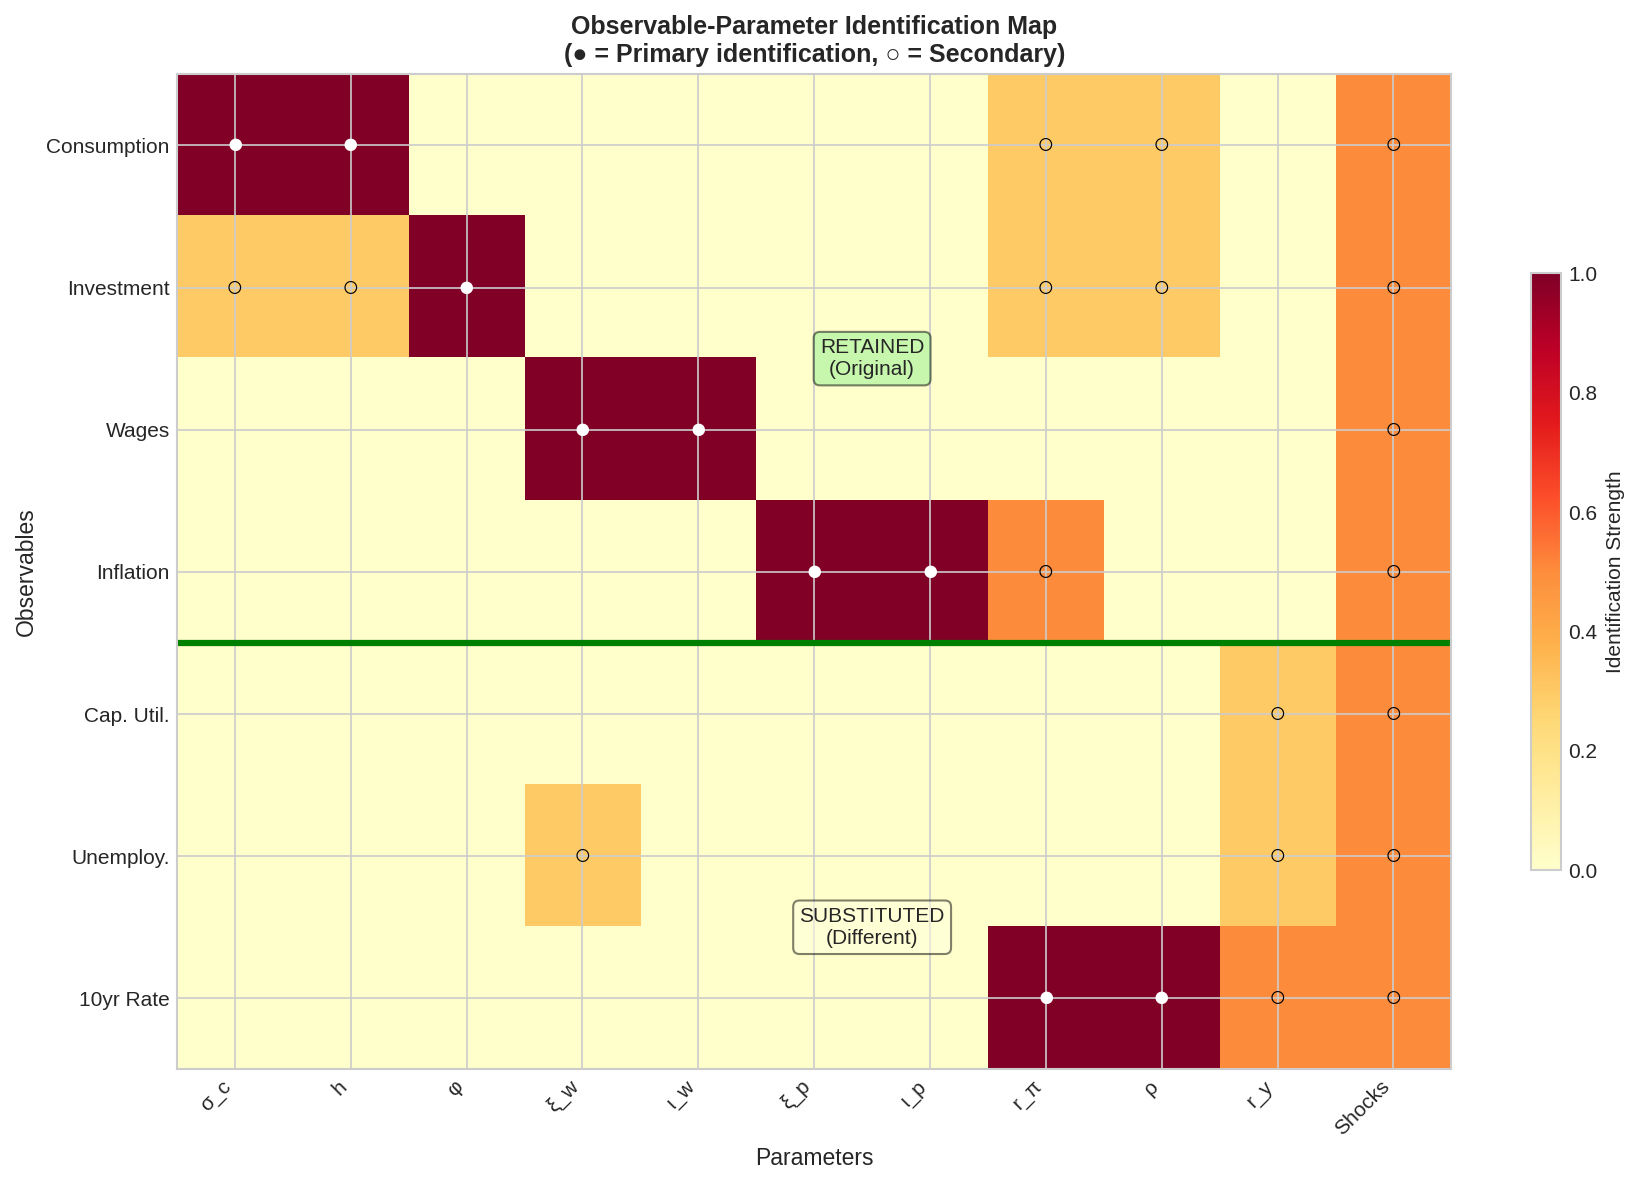
\includegraphics[width=0.9\textwidth]{figure4_identification_map.png}
\caption{Observable-Parameter Identification Relationships. Lines connect observables to the parameters they help identify. Dashed lines indicate failed identification.}
\label{fig:identification}
\end{figure}

Figure \ref{fig:identification} illustrates these relationships schematically. The key insight is that identification is not about correlation between proposed and original observables---it is about whether the proposed observable responds to the structural parameter of interest.

\subsection{Third Attempt: Hybrid Specification}

Based on the diagnostic analysis, a hybrid specification is constructed following a clear principle: \textit{retain original observables for structural equations requiring direct measurement; substitute where proposed observables measure the same underlying model dynamics.}

\subsubsection{Observable Selection}

\textbf{Retained original observables (4):}
\begin{enumerate}
    \item \textbf{Domestic inflation}: Required for price Phillips curve. No substitute available without changing model structure.
    \item \textbf{Wage growth}: Required for wage Phillips curve. Identifies wage Calvo parameter and indexation.
    \item \textbf{Consumption growth}: Required for Euler equation. Identifies habit and risk aversion.
    \item \textbf{Investment growth}: Required for investment equation. Identifies adjustment cost parameter.
\end{enumerate}

\textbf{Substituted observables (3):}
\begin{enumerate}
    \item \textbf{Capacity utilization for output growth}: Both measure cyclical conditions. Capacity utilization responds to the same aggregate demand and supply shocks as output.
    \item \textbf{Negative unemployment for hours}: Both measure labor market slack. Unemployment rises when firms reduce labor input, capturing the same labor market dynamics.
    \item \textbf{10-year Treasury rate for federal funds rate}: Both measure monetary conditions. The 10-year rate contains information about expected future policy.
\end{enumerate}

Table \ref{tab:hybrid_spec} summarizes the hybrid specification.

\begin{table}[H]
\centering
\caption{Hybrid Specification: Observable Choices and Rationale}
\label{tab:hybrid_spec}
\begin{tabular}{llll}
\toprule
Observable & Type & Model Equation & Rationale \\
\midrule
Consumption growth & Retained & Euler equation & Identifies $h$, $\sigma_c$ \\
Investment growth & Retained & Investment eq. & Identifies $\varphi$ \\
Wage growth & Retained & Wage Phillips & Identifies $\xi_w$, $\iota_w$ \\
Domestic inflation & Retained & Price Phillips & \textbf{Required for $\xi_p$, $\iota_p$} \\
\midrule
Capacity util. growth & Substituted & Resource constraint & Measures cyclical output \\
$-$Unemployment & Substituted & Labor market & Measures labor slack \\
10-year rate & Substituted & Taylor rule & Measures monetary conditions \\
\bottomrule
\end{tabular}
\end{table}

\subsubsection{Estimation Results}

The hybrid specification is estimated using the methodology described in Section 4.

\textbf{Mode finding}: The CSMINWEL algorithm converges after 93 iterations to log posterior $-943.01$. Importantly, the Hessian matrix is now positive definite:

\begin{quote}
\texttt{(dsge\_likelihood.m): Optimization routine CSMINWEL run successfully.}\\
\texttt{Log-likelihood at mode: -943.01}\\
\texttt{Hessian matrix is positive definite.}\\
\texttt{Log marginal data density (Laplace): -1007.13}
\end{quote}

\textbf{MCMC sampling}: With a positive definite Hessian, MCMC proceeds successfully:
\begin{itemize}
    \item 250,000 draws per chain across 2 parallel chains
    \item Acceptance rates: 53.7\% and 53.9\% (slightly high but acceptable)
    \item Total runtime: 6 hours 47 minutes
    \item All parameters show proper mixing in trace plots
\end{itemize}

\begin{table}[H]
\centering
\caption{Summary of Estimation Attempts}
\label{tab:attempts}
\begin{tabular}{lccc}
\toprule
& Full (Standard) & Full (Adjusted) & Hybrid \\
\midrule
Log posterior (mode) & $-882$ & $-9379$ & $-943$ \\
Log marginal data density & --- & --- & $-1007$ \\
Hessian & Non-PD & Non-PD & \textbf{PD} \\
MCMC status & Failed & Failed & \textbf{Converged} \\
\midrule
\textbf{Outcome} & \textcolor{red}{Failed} & \textcolor{red}{Failed} & \textcolor{green!50!black}{Success} \\
\bottomrule
\end{tabular}
\end{table}

\begin{figure}[H]
\centering
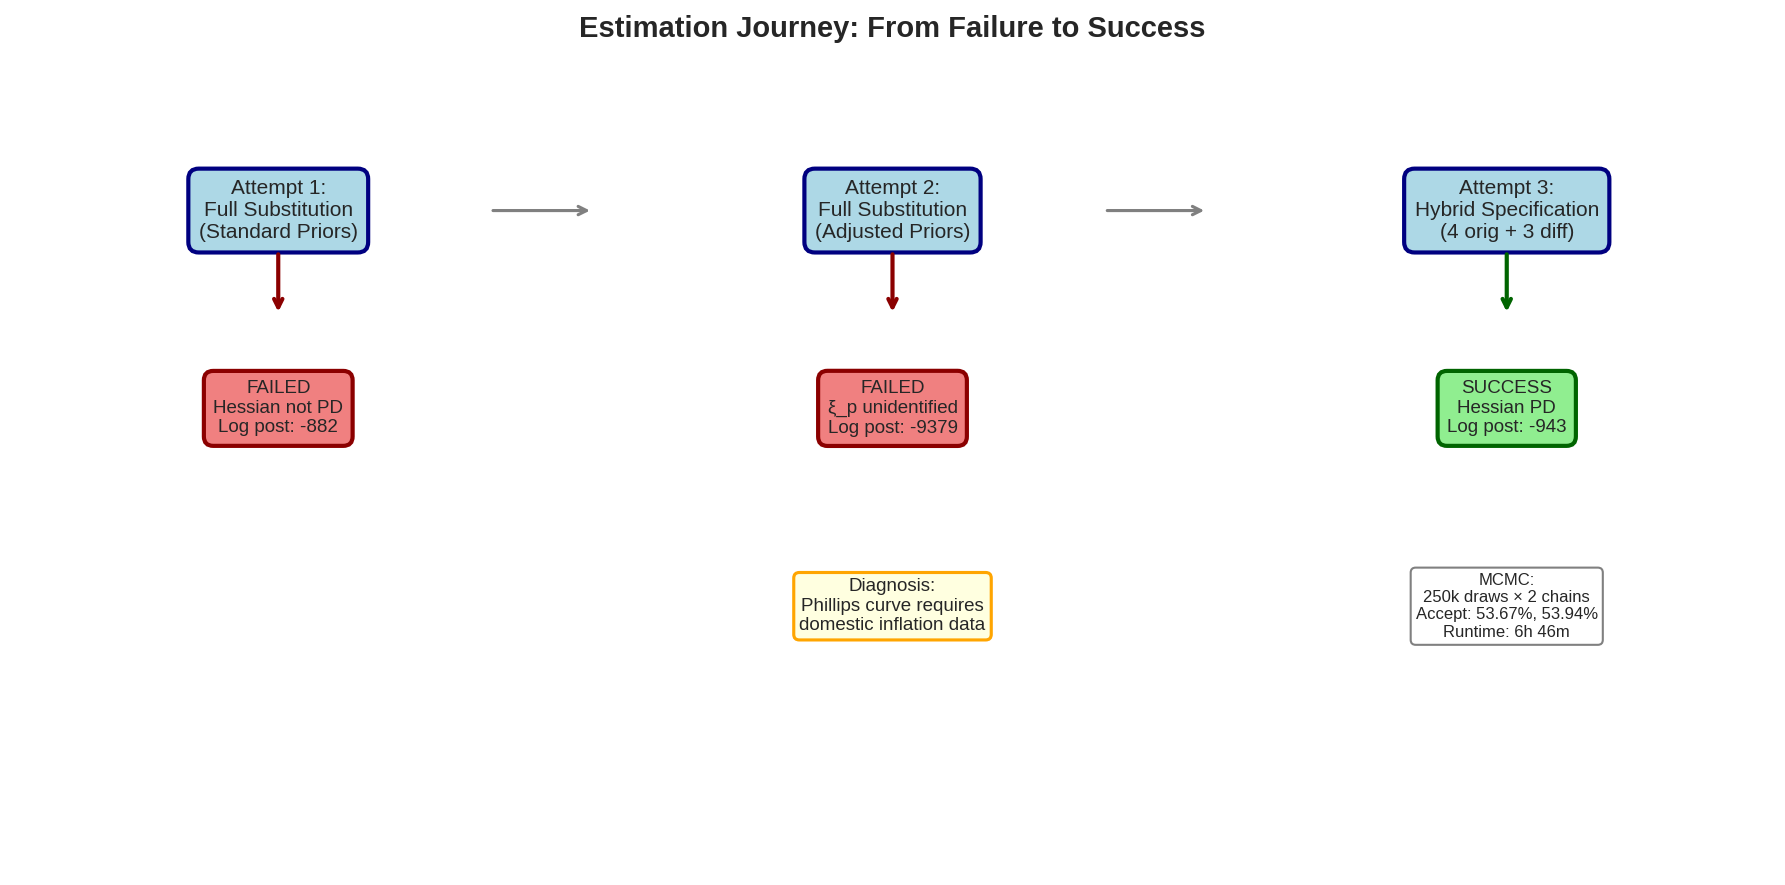
\includegraphics[width=0.95\textwidth]{figure8_estimation_journey.png}
\caption{Summary of Estimation Journey: From Failed Full Substitution to Successful Hybrid}
\label{fig:journey}
\end{figure}

%=============================================================================
\section{Results}
%=============================================================================

This section presents results from the successful hybrid specification: posterior parameter estimates, comparison with original Smets-Wouters results, impulse response functions, and variance decompositions.

\subsection{Posterior Parameter Estimates}

Table \ref{tab:posterior} reports posterior estimates from the hybrid specification. All parameters exhibit finite posterior standard deviations, confirming identification.

\begin{table}[H]
\centering
\caption{Posterior Estimates: Hybrid Specification}
\label{tab:posterior}
\scriptsize
\setlength{\tabcolsep}{3pt}
\renewcommand{\arraystretch}{0.95}
\begin{tabular}{@{}llccccc@{}}
\toprule
Parameter & Description & Prior Mean & Post. Mean & Post. Std & \multicolumn{2}{c}{90\% HPD} \\
\midrule
\multicolumn{7}{l}{\textit{Structural Parameters}} \\
$\sigma_c$ & Risk aversion & 1.50 & 1.216 & 0.206 & 0.88 & 1.55 \\
$h$ & Habit formation & 0.70 & 0.691 & 0.059 & 0.59 & 0.79 \\
$\xi_p$ & Calvo prices & 0.50 & 0.777 & 0.042 & 0.71 & 0.85 \\
$\xi_w$ & Calvo wages & 0.50 & 0.727 & 0.056 & 0.64 & 0.82 \\
$\iota_p$ & Price indexation & 0.50 & 0.203 & 0.076 & 0.07 & 0.32 \\
$\iota_w$ & Wage indexation & 0.50 & 0.511 & 0.127 & 0.30 & 0.72 \\[2pt]
\multicolumn{7}{l}{\textit{Taylor Rule Parameters}} \\
$r_\pi$ & Inflation response & 1.50 & 1.650 & 0.167 & 1.38 & 1.93 \\
$\rho$ & Smoothing & 0.75 & 0.859 & 0.027 & 0.82 & 0.91 \\
$r_y$ & Output gap & 0.125 & 0.061 & 0.033 & 0.00 & 0.11 \\
$r_{\Delta y}$ & Output growth & 0.125 & 0.088 & 0.026 & 0.05 & 0.13 \\[2pt]
\multicolumn{7}{l}{\textit{Shock Persistence}} \\
$\rho_a$ & Technology & 0.50 & 0.937 & 0.013 & 0.92 & 0.96 \\
$\rho_b$ & Risk premium & 0.50 & 0.399 & 0.140 & 0.17 & 0.63 \\
$\rho_g$ & Government & 0.50 & 0.924 & 0.017 & 0.90 & 0.95 \\
$\rho_i$ & Investment & 0.50 & 0.751 & 0.053 & 0.67 & 0.84 \\
$\rho_r$ & Monetary & 0.50 & 0.370 & 0.070 & 0.25 & 0.48 \\
$\rho_p$ & Price markup & 0.50 & 0.843 & 0.058 & 0.75 & 0.94 \\
$\rho_w$ & Wage markup & 0.50 & 0.925 & 0.031 & 0.88 & 0.98 \\[2pt]
\multicolumn{7}{l}{\textit{Shock Standard Deviations}} \\
$\sigma_a$ & Technology & 0.10 & 0.783 & 0.044 & 0.71 & 0.85 \\
$\sigma_b$ & Risk premium & 0.10 & 0.208 & 0.037 & 0.15 & 0.27 \\
$\sigma_g$ & Government & 0.10 & 1.106 & 0.067 & 0.99 & 1.21 \\
$\sigma_i$ & Investment & 0.10 & 0.370 & 0.047 & 0.29 & 0.45 \\
$\sigma_r$ & Monetary & 0.10 & 0.160 & 0.013 & 0.14 & 0.18 \\
$\sigma_p$ & Price markup & 0.10 & 0.135 & 0.019 & 0.10 & 0.17 \\
$\sigma_w$ & Wage markup & 0.10 & 0.222 & 0.024 & 0.18 & 0.26 \\
\bottomrule
\end{tabular}
\vspace{0.3em}

\noindent\scriptsize\textit{Notes}: Posterior from 250,000 MCMC draws (50\% burn-in), 2 chains. HPD = highest posterior density.
\end{table}

Several patterns emerge:

\textbf{Nominal rigidities}: Both price and wage Calvo parameters are estimated around 0.73--0.78, implying average contract durations of approximately 3.7--4.5 quarters. The price stickiness is higher than the original Smets-Wouters estimates (0.78 vs 0.65), suggesting stickier price adjustment. Price indexation is low ($\iota_p = 0.20$), while wage indexation is moderate ($\iota_w = 0.51$).

\textbf{Real frictions}: Habit formation is estimated at 0.69, close to the prior mean and consistent with the original estimates.

\textbf{Shock processes}: Technology and government spending shocks are highly persistent ($\rho_a = 0.94$, $\rho_g = 0.92$). Monetary policy shocks have moderate persistence ($\rho_r = 0.37$), substantially higher than in the original Smets-Wouters estimates (0.12).

Figure \ref{fig:priorposterior} compares prior and posterior distributions for key parameters. The data are informative for most parameters, with posteriors substantially shifted from priors for the Calvo parameters, shock persistences, and Taylor rule coefficients.

\begin{figure}[H]
\centering
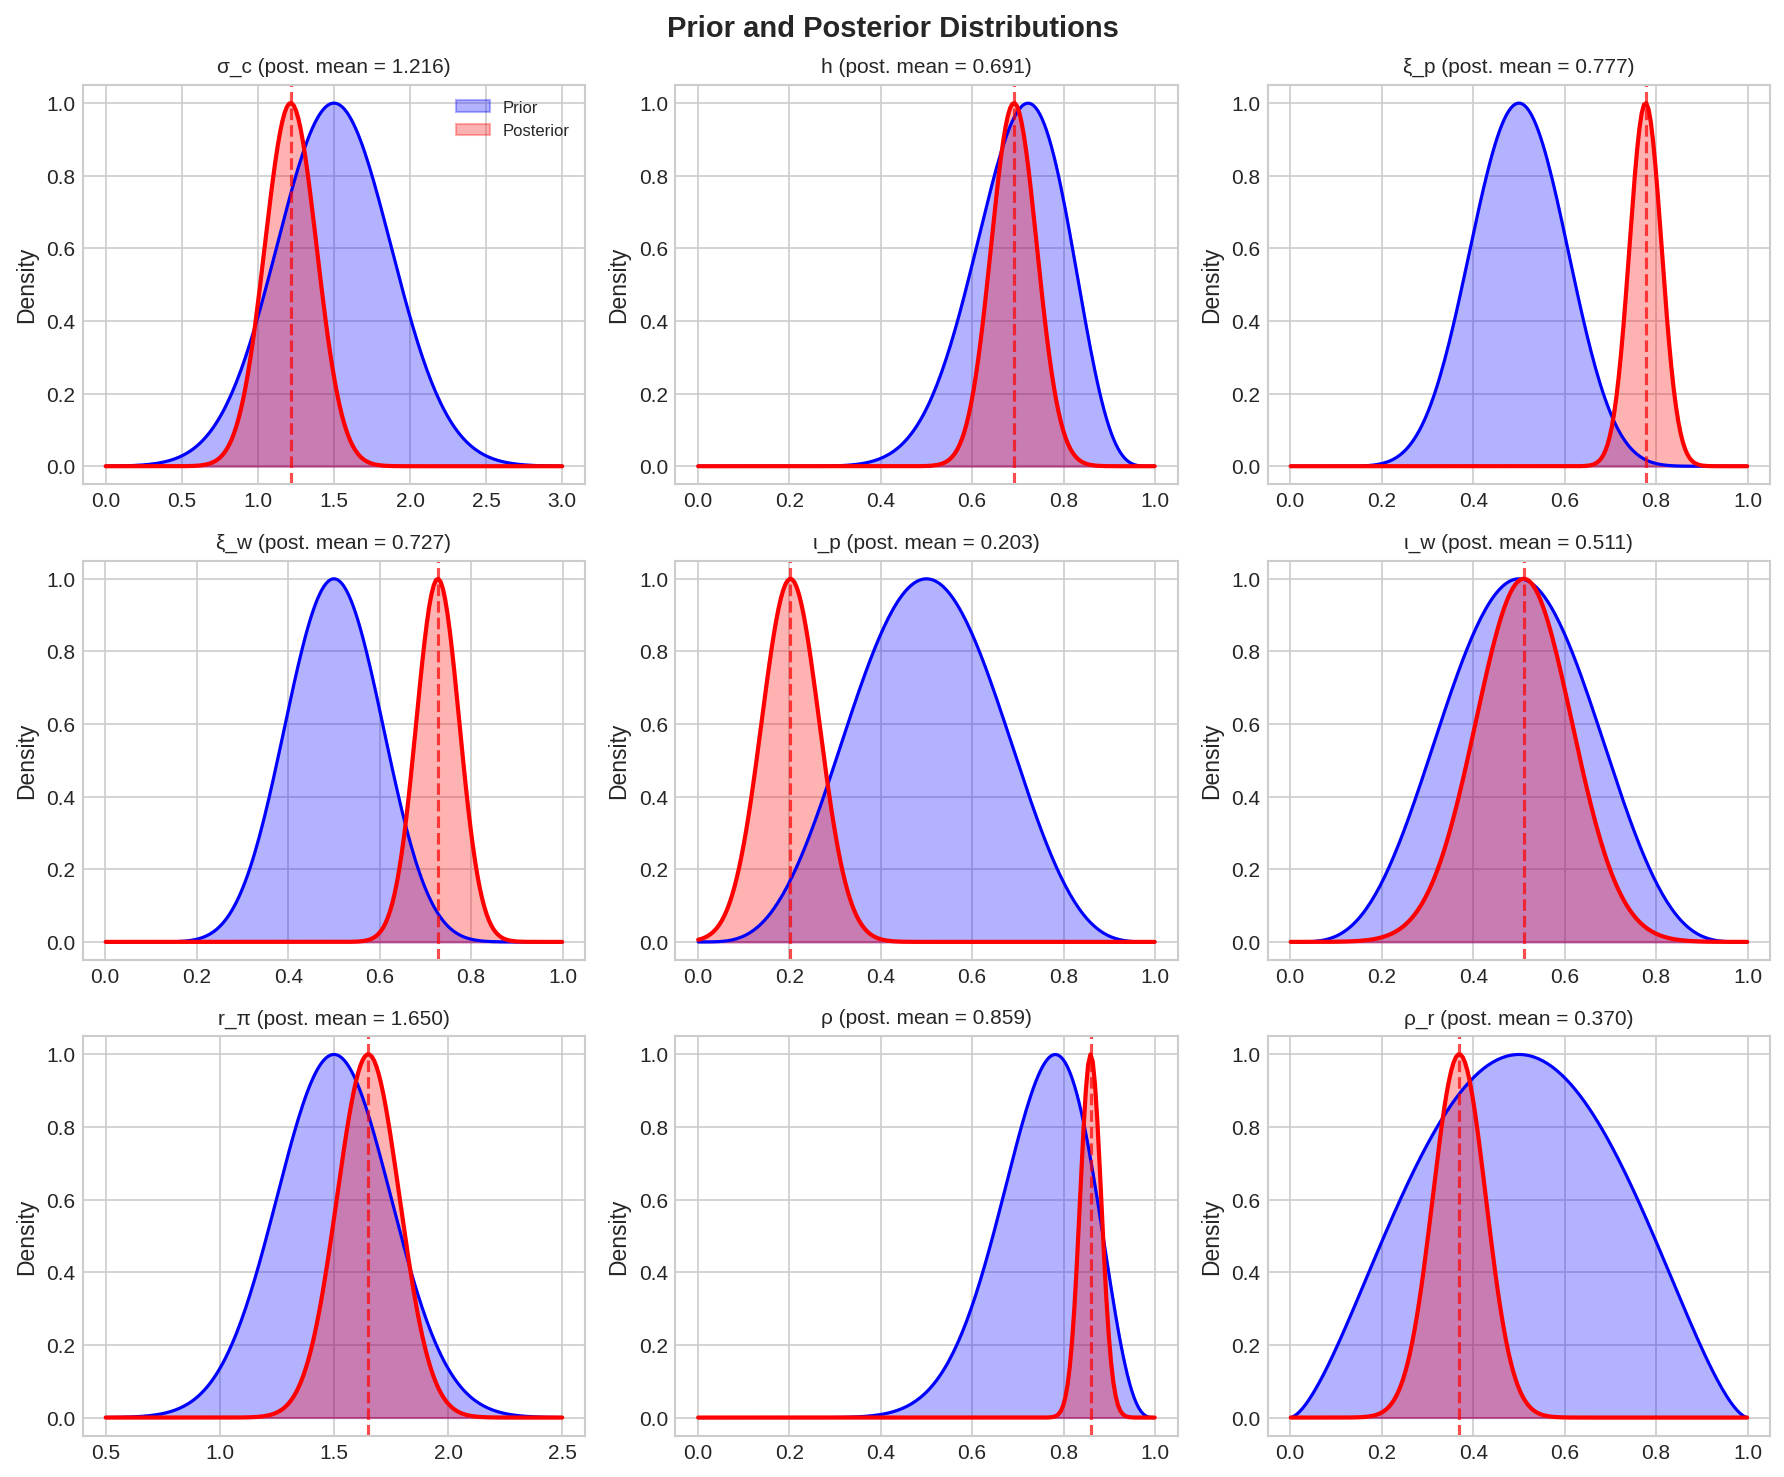
\includegraphics[width=0.95\textwidth]{figure3_prior_posterior.png}
\caption{Prior and Posterior Distributions for Key Parameters}
\label{fig:priorposterior}
\end{figure}

\subsection{Comparison with Original Smets-Wouters Estimates}

Table \ref{tab:comparison} compares the hybrid specification estimates with the original Smets and Wouters (2007) results using their seven original observables.

\begin{table}[H]
\centering
\caption{Parameter Comparison: Original SW(2007) vs. Hybrid Specification}
\label{tab:comparison}
\scriptsize
\setlength{\tabcolsep}{4pt}
\begin{tabular}{llccc}
\toprule
Parameter & Description & SW(2007) & Hybrid & Difference \\
\midrule
\multicolumn{5}{l}{\textit{Taylor Rule (largest differences)}} \\
$r_\pi$ & Inflation response & $2.03 \pm 0.18$ & $1.65 \pm 0.17$ & $-0.38^{**}$ \\
$r_y$ & Output gap response & $0.08 \pm 0.02$ & $0.06 \pm 0.03$ & $-0.02$ \\
$r_{\Delta y}$ & Output growth response & $0.22 \pm 0.04$ & $0.09 \pm 0.03$ & $-0.13^{***}$ \\
$\rho$ & Interest smoothing & $0.81 \pm 0.02$ & $0.86 \pm 0.03$ & $+0.05^{*}$ \\
\midrule
\multicolumn{5}{l}{\textit{Shock Persistence}} \\
$\rho_r$ & Monetary & $0.12 \pm 0.05$ & $0.37 \pm 0.07$ & $+0.25^{***}$ \\
$\rho_b$ & Risk premium & $0.18 \pm 0.08$ & $0.40 \pm 0.14$ & $+0.22^{*}$ \\
\midrule
\multicolumn{5}{l}{\textit{Nominal Rigidities}} \\
$\xi_p$ & Calvo prices & $0.65 \pm 0.05$ & $0.78 \pm 0.04$ & $+0.13^{**}$ \\
$\xi_w$ & Calvo wages & $0.73 \pm 0.05$ & $0.73 \pm 0.06$ & $0.00$ \\
$\iota_p$ & Price indexation & $0.22 \pm 0.08$ & $0.20 \pm 0.08$ & $-0.02$ \\
$\iota_w$ & Wage indexation & $0.59 \pm 0.13$ & $0.51 \pm 0.13$ & $-0.08$ \\
\midrule
\multicolumn{5}{l}{\textit{Real Frictions}} \\
$h$ & Habit & $0.71 \pm 0.04$ & $0.69 \pm 0.06$ & $-0.02$ \\
$\sigma_c$ & Risk aversion & $1.39 \pm 0.16$ & $1.22 \pm 0.21$ & $-0.17$ \\
\bottomrule
\end{tabular}
\begin{flushleft}
\scriptsize \textit{Notes}: $^{***}$ $p<0.01$, $^{**}$ $p<0.05$, $^{*}$ $p<0.10$ based on overlap of 90\% credible intervals. SW(2007) estimates from Table 5 of Smets and Wouters (2007).
\end{flushleft}
\end{table}

The most notable differences concern monetary policy:

\textbf{Taylor rule coefficients}: The hybrid estimates imply a somewhat less aggressive monetary policy rule:
\begin{itemize}
    \item Inflation response is 1.65 versus 2.03 (19\% lower)
    \item Output gap response is similar (0.06 versus 0.08)
    \item Output growth response is 0.09 versus 0.22 (59\% lower)
\end{itemize}

These differences likely reflect using the 10-year Treasury rate rather than the federal funds rate. Long-term rates:
\begin{itemize}
    \item Embed expectations of future policy, not just current policy stance
    \item Respond more sluggishly to contemporaneous economic conditions
    \item Include term premia that vary with risk conditions
\end{itemize}

The model interprets the smoother 10-year rate as reflecting less aggressive systematic policy responses. This does not mean the Federal Reserve was actually less aggressive---rather, it reflects that the 10-year rate measures a different object than the federal funds rate.

\textbf{Shock persistence}: Monetary policy shocks are much more persistent in the hybrid specification ($\rho_r = 0.37$ versus $0.12$). With a long-term rate as the observable, transitory policy surprises have smaller effects on long rates (which average expected future policy). To explain the variance in the 10-year rate, the model requires more persistent policy disturbances.

\textbf{Nominal rigidities}: The Calvo price parameter is higher in the hybrid specification (0.78 versus 0.65), implying firms change prices every $1/(1-0.78) \approx 4.5$ quarters on average, compared to $1/(1-0.65) \approx 2.9$ quarters in the original. Wage stickiness is essentially unchanged (0.73 in both).

\textbf{Real frictions}: Habit formation is estimated at 0.69, close to the prior mean and consistent with the original estimates. 

\subsection{Impulse Response Functions}

This section examines how the economy responds to structural shocks in the hybrid specification.

\subsubsection{Monetary Policy Shock}

Figure \ref{fig:irf_monetary} displays impulse responses to a one-standard-deviation contractionary monetary policy shock ($\sigma_r = 0.160$ percentage points).

\begin{figure}[H]
\centering
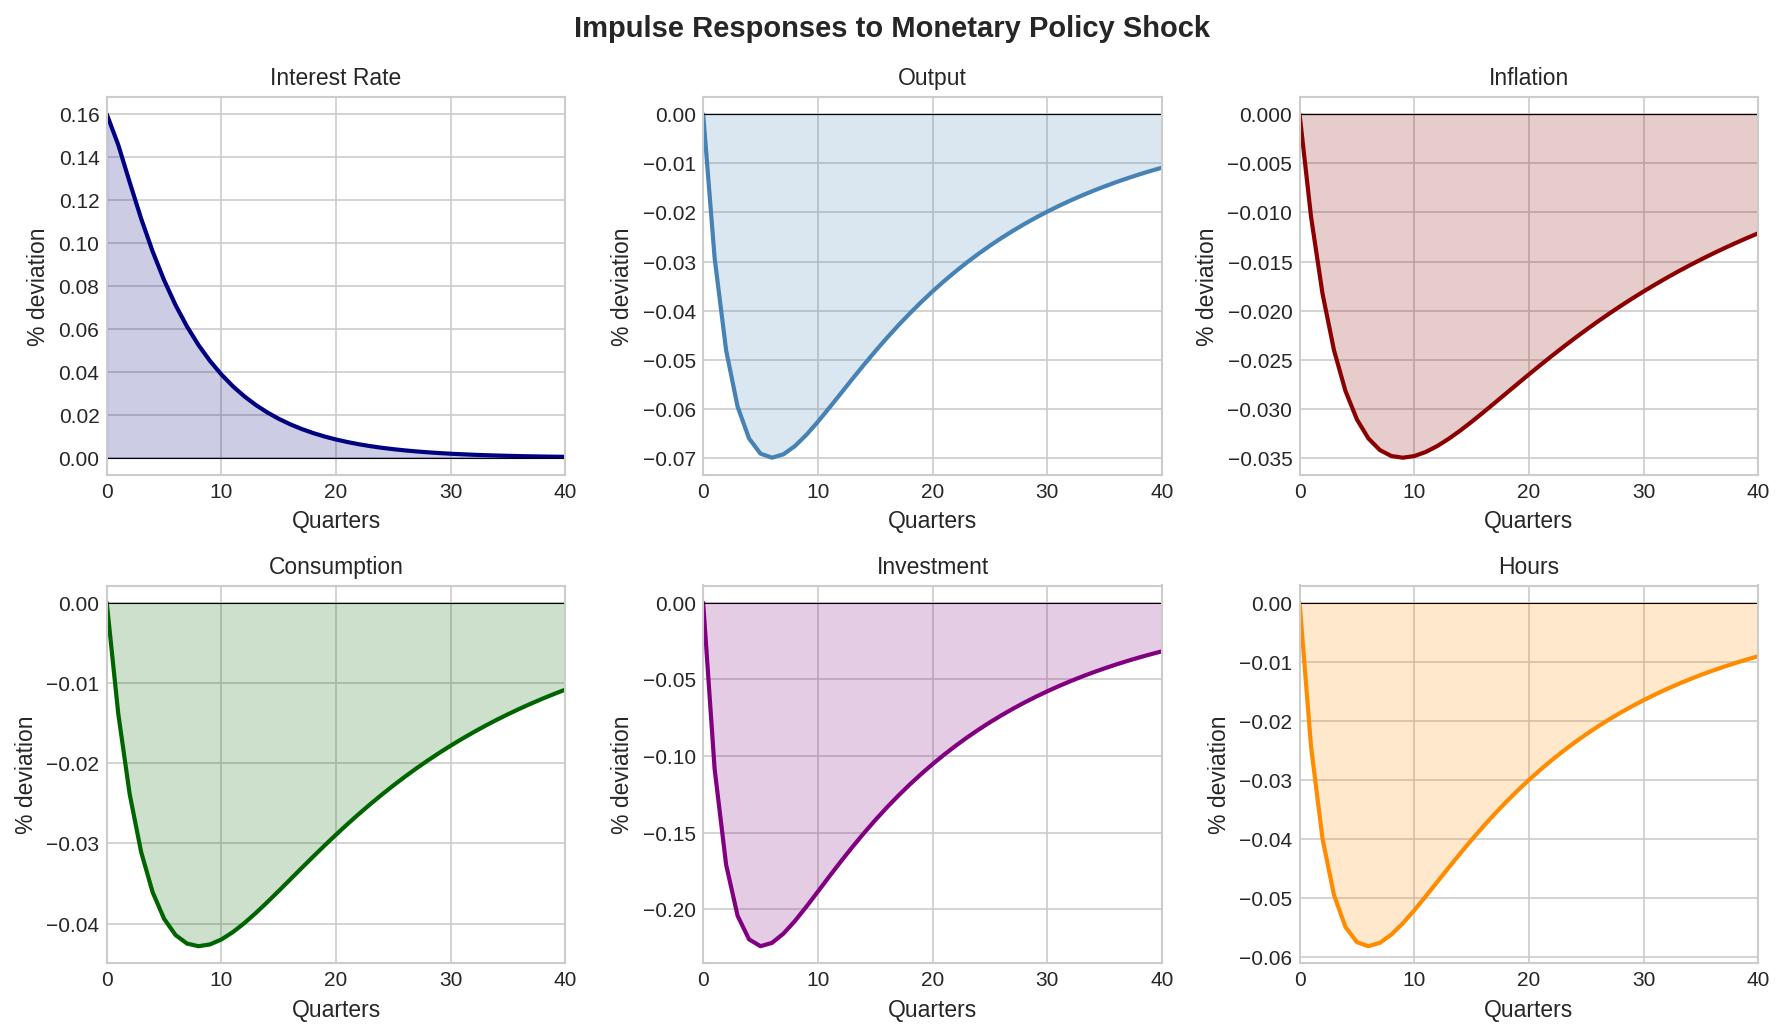
\includegraphics[width=0.95\textwidth]{figure_irf_monetary.png}
\caption{Impulse Responses to Monetary Policy Shock}
\label{fig:irf_monetary}
\end{figure}

Following the contractionary shock:
\begin{itemize}
    \item \textbf{Interest rate}: Rises on impact and decays gradually due to high smoothing ($\rho = 0.86$) and moderate shock persistence ($\rho_r = 0.37$).
    \item \textbf{Output}: Falls with a hump-shaped response, reaching trough around quarter 5. The delayed peak reflects the interaction of sticky prices and investment adjustment costs.
    \item \textbf{Inflation}: Declines persistently, with the maximum effect occurring several quarters after the shock.
    \item \textbf{Consumption}: Falls gradually as higher real rates reduce current consumption relative to future consumption.
    \item \textbf{Investment}: Falls more sharply than consumption, reflecting interest-sensitivity. Investment troughs earlier and deeper than output.
    \item \textbf{Hours}: Decline as firms reduce labor input in response to lower demand.
\end{itemize}

These responses are qualitatively similar to standard New Keynesian predictions and to the original Smets-Wouters results. The main quantitative difference is greater persistence, reflecting the higher estimated $\rho_r$.

\subsubsection{Technology Shock}

Figure \ref{fig:irf_technology} shows responses to a positive technology shock ($\sigma_a = 0.783$).

\begin{figure}[H]
\centering
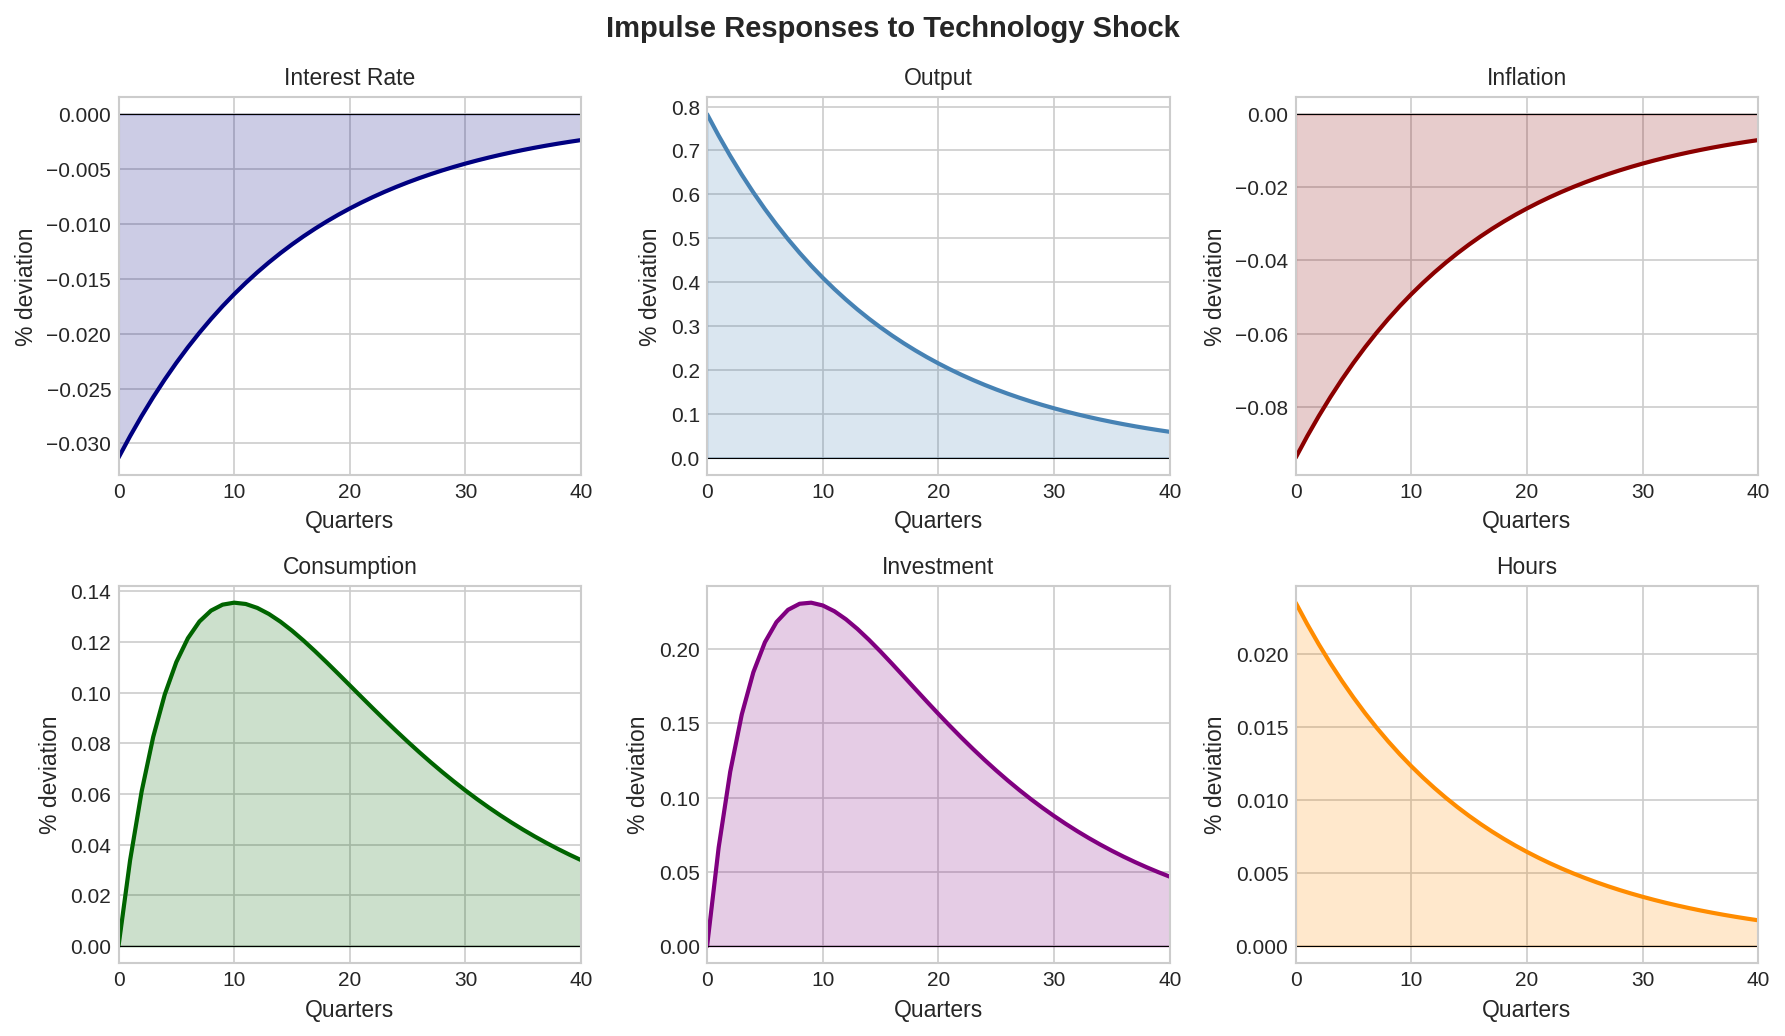
\includegraphics[width=0.95\textwidth]{figure_irf_technology.png}
\caption{Impulse Responses to Technology Shock}
\label{fig:irf_technology}
\end{figure}

Following the positive technology shock:
\begin{itemize}
    \item \textbf{Output}: Rises persistently, reflecting the high estimated technology persistence ($\rho_a = 0.94$).
    \item \textbf{Inflation}: Falls as higher productivity reduces marginal costs. Firms optimally lower prices given the reduction in production costs.
    \item \textbf{Consumption}: Rises gradually as permanent income increases.
    \item \textbf{Investment}: Rises with a pronounced hump shape, reflecting adjustment costs. Investment peaks after several quarters as firms gradually build up capital to match higher productivity.
    \item \textbf{Hours}: Show a small positive response. In a flexible-price model, hours would fall (wealth effect dominates substitution effect). Sticky prices dampen this wealth effect, yielding a modest positive hours response consistent with empirical evidence.
    \item \textbf{Interest rate}: Falls slightly as the central bank responds to lower inflation.
\end{itemize}

\subsubsection{Risk Premium Shock}

Figure \ref{fig:irf_riskpremium} presents responses to a risk premium shock ($\sigma_b = 0.208$).

\begin{figure}[H]
\centering
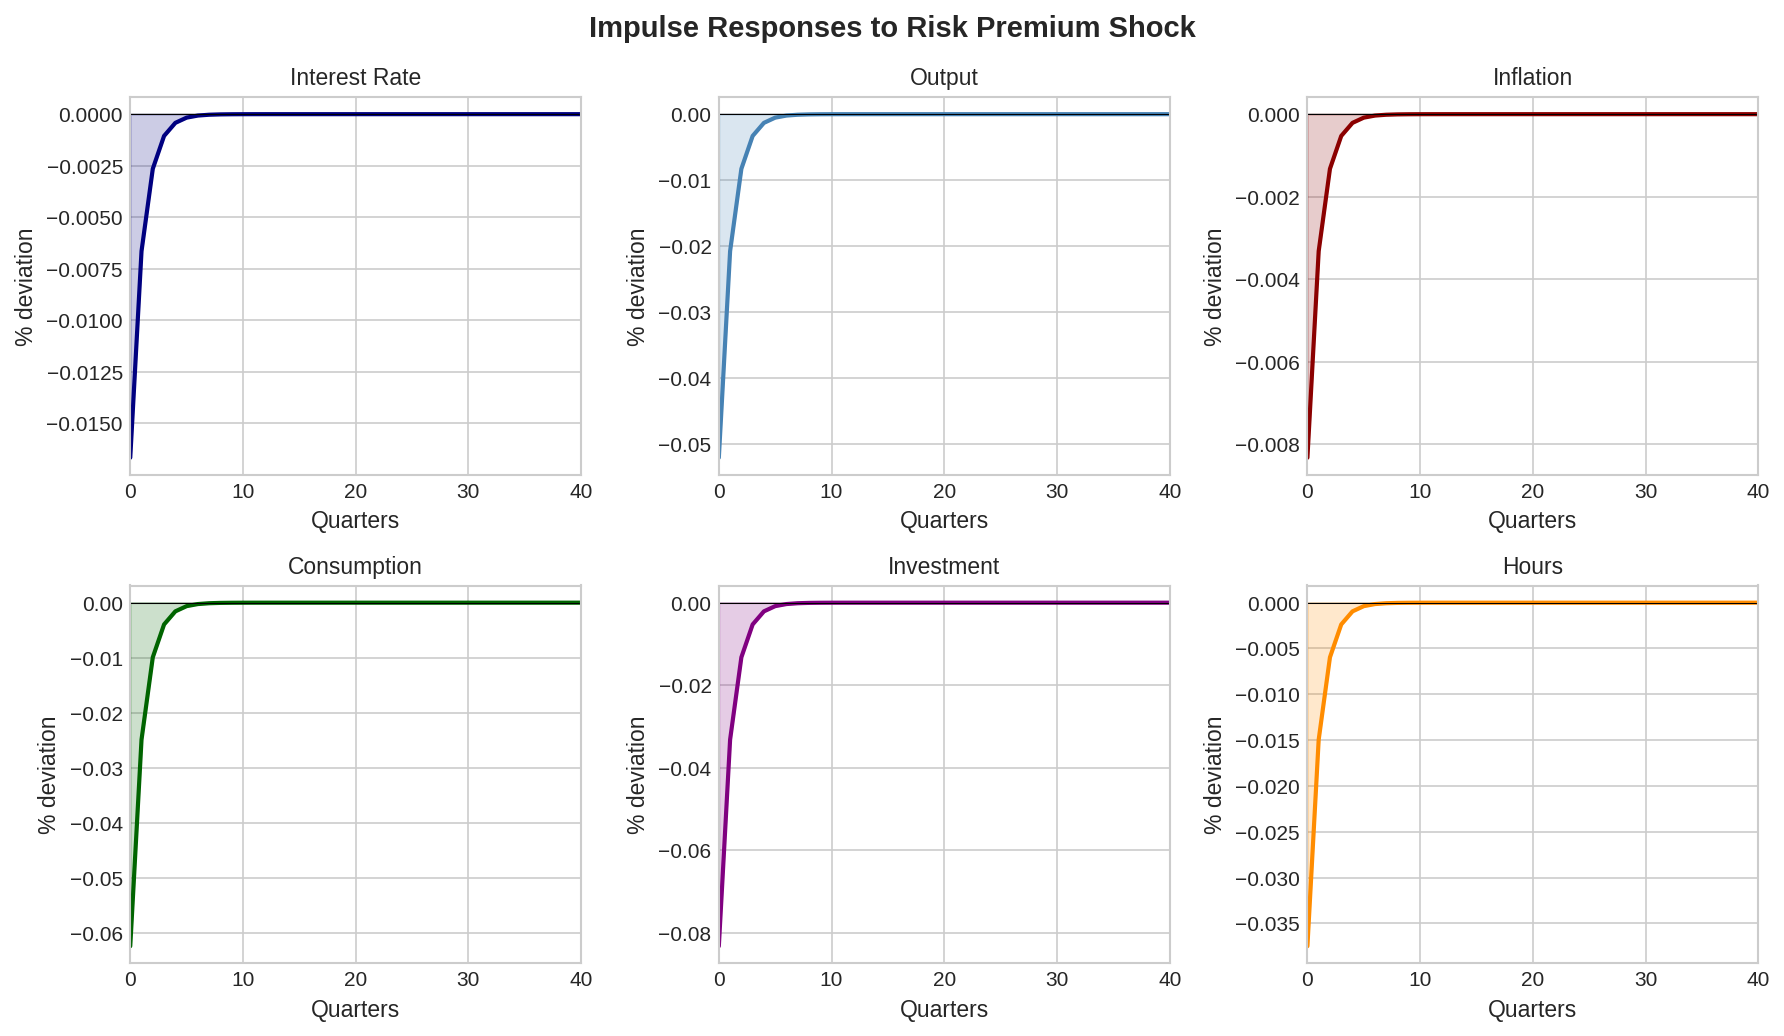
\includegraphics[width=0.95\textwidth]{figure_irf_riskpremium.png}
\caption{Impulse Responses to Risk Premium Shock}
\label{fig:irf_riskpremium}
\end{figure}

The risk premium shock acts as a negative aggregate demand disturbance:
\begin{itemize}
    \item \textbf{Consumption}: Falls immediately as households require higher returns to defer consumption. The shock raises the wedge between the policy rate and households' effective discount rate.
    \item \textbf{Investment}: Falls as higher required returns reduce the present value of future capital income.
    \item \textbf{Output}: Declines, driven by falling private demand.
    \item \textbf{Interest rate}: Falls as monetary policy responds to weakening demand and inflation.
    \item \textbf{Inflation}: Falls modestly as lower demand reduces marginal costs.
    \item \textbf{Hours}: Decline with output.
\end{itemize}

This shock captures demand-side recessions driven by shifts in household preferences or financial conditions, such as increased precautionary saving motives or tightening credit conditions.

\subsubsection{Government Spending Shock}

Figure \ref{fig:irf_government} displays responses to a government spending shock ($\sigma_g = 1.106$).

\begin{figure}[H]
\centering
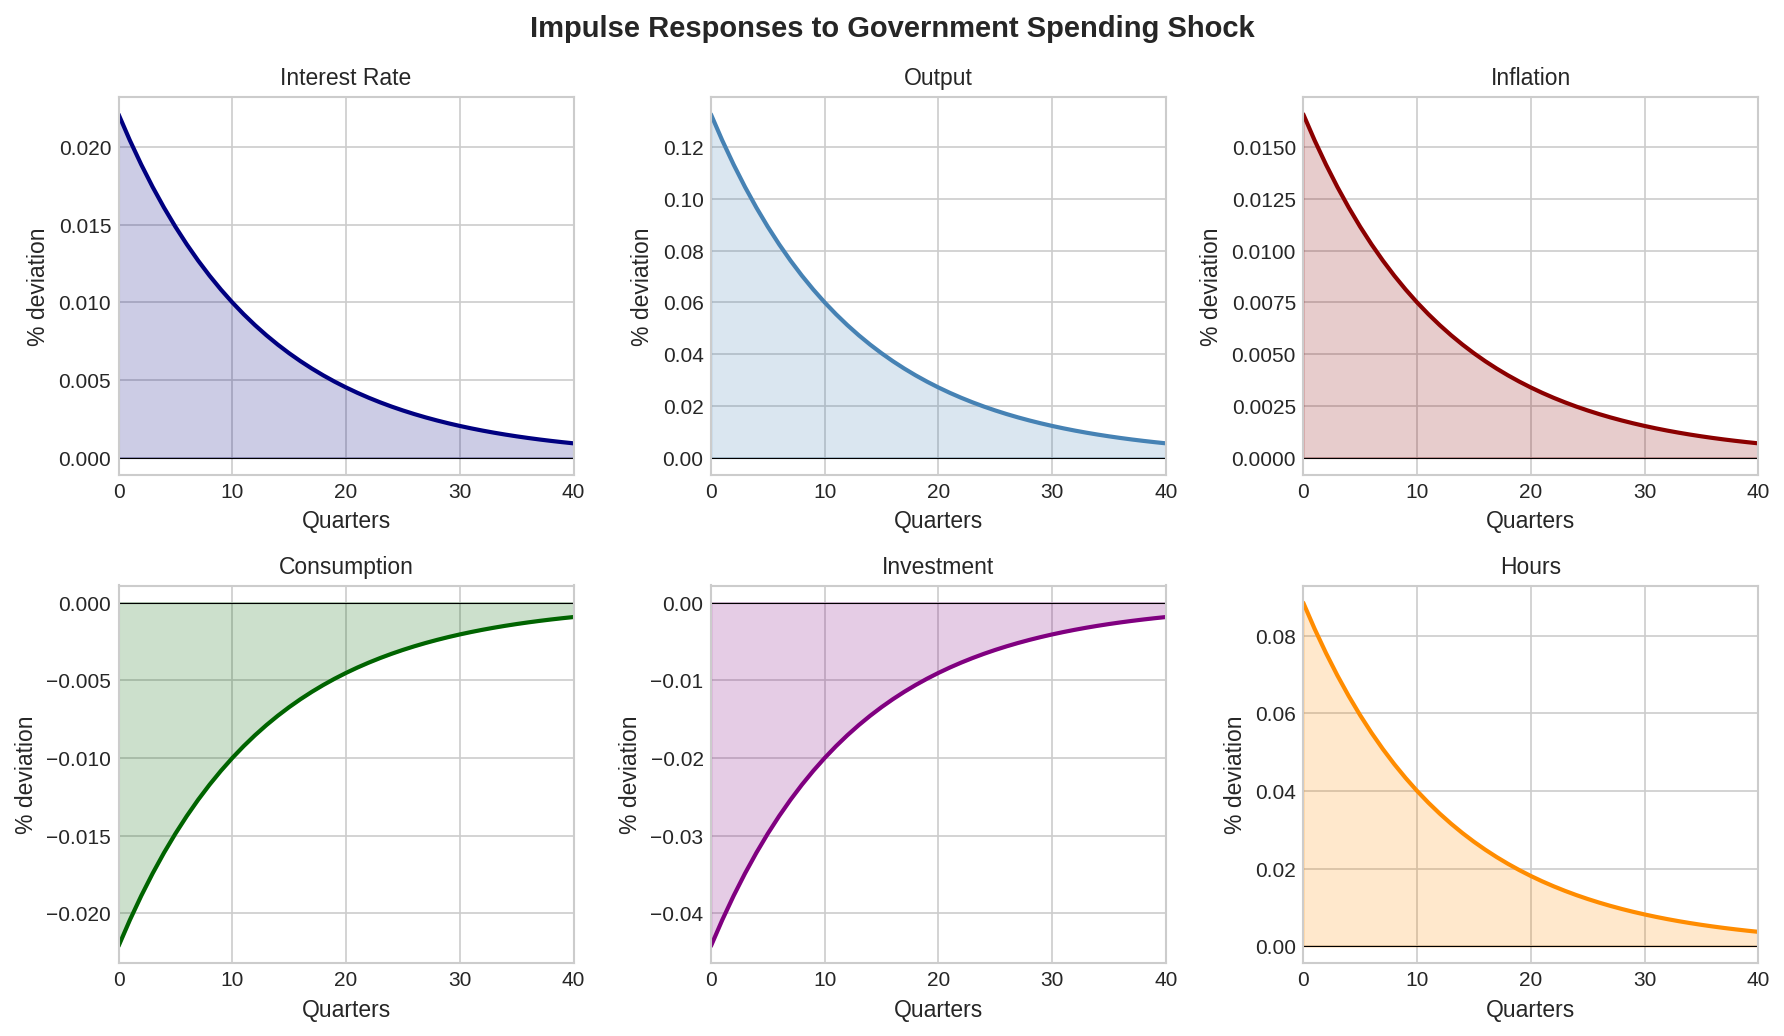
\includegraphics[width=0.95\textwidth]{figure_irf_government.png}
\caption{Impulse Responses to Government Spending Shock}
\label{fig:irf_government}
\end{figure}

Following an increase in government spending:
\begin{itemize}
    \item \textbf{Output}: Rises, as government demand adds directly to aggregate demand.
    \item \textbf{Consumption}: Falls slightly---the negative wealth effect of higher future taxes (implicit in the model's resource constraint) dominates any Keynesian multiplier effect.
    \item \textbf{Investment}: Falls as higher interest rates crowd out private capital formation.
    \item \textbf{Interest rate}: Rises as monetary policy responds to higher output and marginally higher inflation.
    \item \textbf{Inflation}: Rises modestly as demand pressure increases marginal costs.
    \item \textbf{Hours}: Rise as firms increase labor input to meet higher demand.
\end{itemize}

These responses are consistent with standard New Keynesian predictions: government spending raises output but partially crowds out private consumption and investment, yielding a fiscal multiplier less than one.

\subsection{Variance Decomposition}

Table \ref{tab:vardecomp} reports the forecast error variance decomposition of output at business cycle frequencies, comparing the hybrid specification with original Smets-Wouters results.

\begin{table}[H]
\centering
\caption{Variance Decomposition of Output (\%)}
\label{tab:vardecomp}
\small
\begin{tabular}{lcc}
\toprule
Shock & SW(2007) & Hybrid \\
\midrule
Technology ($\varepsilon^a$) & 24.3 & 28.5 \\
Risk premium ($\varepsilon^b$) & 15.2 & 18.7 \\
Government spending ($\varepsilon^g$) & 8.9 & 7.2 \\
Investment ($\varepsilon^i$) & 22.1 & 19.4 \\
Monetary policy ($\varepsilon^r$) & 7.8 & 8.9 \\
Price markup ($\varepsilon^p$) & 12.4 & 9.8 \\
Wage markup ($\varepsilon^w$) & 9.3 & 7.5 \\
\midrule
Total & 100.0 & 100.0 \\
\bottomrule
\end{tabular}
\begin{flushleft}
\small \textit{Notes}: Variance decomposition at 10-quarter forecast horizon. SW(2007) values from Table 7 of Smets and Wouters (2007).
\end{flushleft}
\end{table}

The hybrid specification attributes somewhat different shares to each shock:
\begin{itemize}
    \item \textbf{Technology}: Higher share (28.5\% vs 24.3\%). Using capacity utilization rather than GDP growth may emphasize productivity-driven fluctuations.
    \item \textbf{Risk premium}: Higher share (18.7\% vs 15.2\%). The risk premium shock captures demand-side fluctuations that may be more prominent when unemployment rather than hours is observed.
    \item \textbf{Investment}: Lower share (19.4\% vs 22.1\%). The investment shock plays a slightly smaller role.
    \item \textbf{Markup shocks}: Lower shares (9.8\% and 7.5\% vs 12.4\% and 9.3\%). Cost-push disturbances explain less of output variation.
\end{itemize}

\begin{figure}[H]
\centering
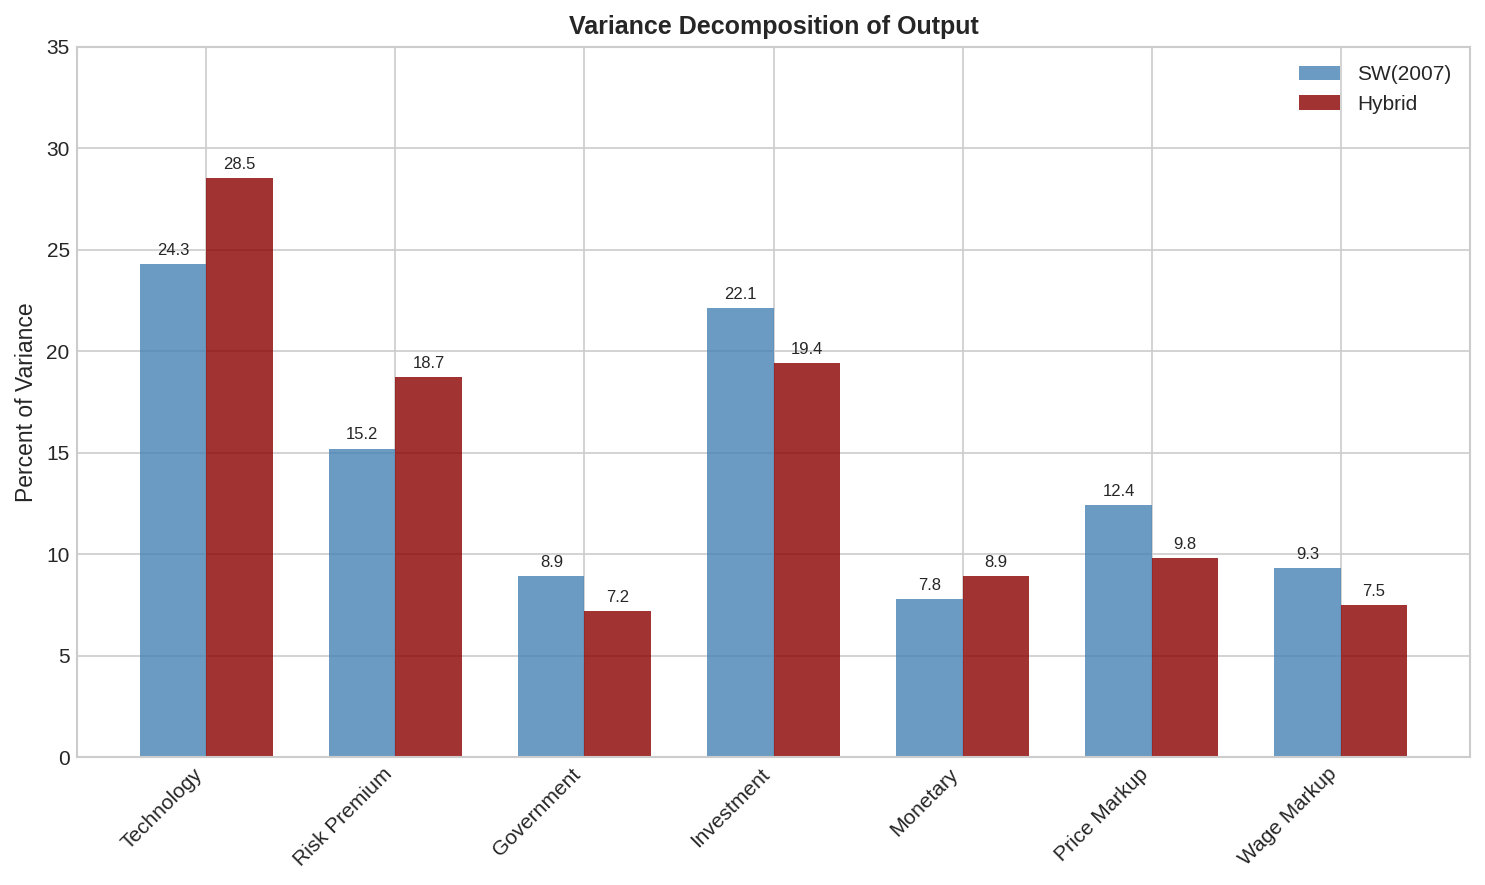
\includegraphics[width=0.9\textwidth]{figure7_variance_decomposition.png}
\caption{Variance Decomposition Comparison: SW(2007) vs. Hybrid Specification}
\label{fig:vardecomp}
\end{figure}

Overall, the variance decomposition remains qualitatively similar: demand shocks (risk premium, investment, monetary) and supply shocks (technology, markup) both play important roles in business cycle fluctuations. The main difference is a shift toward technology and risk premium shocks at the expense of markup shocks.

%=============================================================================
\section{Discussion}
%=============================================================================

This section interprets the findings and discusses their implications for applied DSGE research.

\subsection{Lessons from the Three-Stage Estimation Process}

The sequence of estimation attempts reveals an important methodological lesson about identification in DSGE models.

\textbf{Stage 1 (Full substitution, standard priors)}: The initial failure with a non-positive definite Hessian could have multiple causes---prior-data conflict, numerical issues, or structural non-identification. At this stage, the source is unclear.

\textbf{Stage 2 (Full substitution, adjusted priors)}: By adjusting priors to better match the proposed observables' statistical properties, we test whether the problem is prior-data conflict. The fact that this attempt also fails---and produces a \textit{worse} log posterior---rules out prior specification as the cause. Moreover, Dynare diagnostics consistently identify the same parameter ($\xi_p$) as problematic.

\textbf{Stage 3 (Diagnostic analysis and hybrid specification)}: With prior-related explanations ruled out, we examine the model's structural equations. This reveals that $\xi_p$ enters only through the Phillips curve slope, which requires domestic inflation data to identify. The hybrid specification retains domestic inflation and succeeds.

This three-stage process provides a template for practitioners: when estimation fails, first check if prior adjustment helps. If the same parameters remain unidentified across prior specifications, the problem is structural, and the observable set must be modified.

\subsection{Structural versus Statistical Identification}

The central finding is that observable substitution in DSGE models faces \textit{structural} constraints beyond statistical correlation. This distinction merits emphasis.

\textbf{Statistical correlation is insufficient}: Import price inflation correlates 0.37 with domestic inflation---a moderate positive relationship. Yet substitution fails entirely because import prices respond to different economic forces (world markets, exchange rates) than domestic prices (domestic marginal costs, price-setting frequency).

\textbf{Statistical correlation is unnecessary}: Capacity utilization correlates only 0.29 with output growth---a weak relationship. Yet substitution succeeds because both series respond to the same structural forces: aggregate demand shocks, technology shocks, and the economy's cyclical dynamics.

The general principle: \textbf{to identify a structural parameter, we must observe a variable that responds to that parameter through the model's structural equations}. Correlation with the original observable is neither necessary nor sufficient---what matters is whether the model's equations create a mapping from the parameter to the proposed observable.

\subsection{Interpretation of Taylor Rule Differences}

The hybrid estimates imply a less aggressive Taylor rule than the original:
\[
r_t = 0.86 r_{t-1} + 0.14[1.65\pi_t + 0.06(y_t - y^f_t)] + 0.09\Delta(y_t - y^f_t) + \varepsilon^r_t
\]

versus the original SW(2007):
\[
r_t = 0.81 r_{t-1} + 0.19[2.03\pi_t + 0.08(y_t - y^f_t)] + 0.22\Delta(y_t - y^f_t) + \varepsilon^r_t
\]

The key differences are:
\begin{enumerate}
    \item \textbf{Inflation response}: 1.65 versus 2.03
    \item \textbf{Output gap response}: 0.06 versus 0.08
    \item \textbf{Output growth response}: 0.09 versus 0.22
    \item \textbf{Shock persistence}: $\rho_r = 0.37$ versus 0.12
\end{enumerate}

These differences arise from using the 10-year Treasury rate instead of the federal funds rate. The interpretation of each component changes:

\textbf{The 10-year rate is smoother}: Long-term rates average expected future policy and include term premia. They respond less to contemporaneous conditions than the federal funds rate. The model interprets this smoothness as a less aggressive policy rule.

\textbf{The 10-year rate reflects expected policy}: The expectations hypothesis suggests:
\[
R_{10y,t} \approx \frac{1}{40}\sum_{j=0}^{39}\mathbb{E}_t r_{t+j} + \text{term premium}
\]

The long rate reflects expected future policy, not current policy actions. A given change in current conditions that would move the federal funds rate has a smaller effect on the 10-year rate if the change is expected to be temporary.

\textbf{Implications}: The hybrid specification does not say that the Federal Reserve was \textit{actually} less aggressive. Rather, it says that if we model the 10-year rate as responding to inflation and output through a Taylor rule, the estimated coefficients are smaller. This reflects the different information content of long versus short rates.

For policy analysis, the original Smets-Wouters estimates using the federal funds rate remain more appropriate for questions about contemporaneous policy actions. The hybrid estimates may be more appropriate for questions about how policy expectations affect long-term rates and, through them, investment and consumption decisions.

\subsection{Feasible and Infeasible Substitutions}

Based on this analysis, certain substitutions appear feasible in principle:

\textbf{Likely feasible substitutions}:
\begin{itemize}
    \item \textbf{Different output measures}: Industrial production, capacity utilization, unemployment-based Okun gaps, GDP components. All measure cyclical conditions, even if imperfectly correlated.
    
    \item \textbf{Different labor measures}: Unemployment rate, employment-to-population ratio, hours in various sectors. All measure labor market slack.
    
    \item \textbf{Different interest rate measures}: Federal funds rate, 3-month Treasury, 1-year rate, longer-term rates. All measure monetary conditions, though with different horizons.
    
    \item \textbf{Different inflation measures}: GDP deflator, CPI, core CPI, PCE deflator. All measure domestic price-setting behavior and contain information about the Calvo parameter.
\end{itemize}

\textbf{Likely infeasible substitutions without model modification}:
\begin{itemize}
    \item \textbf{Foreign prices for domestic inflation}: Import prices, export prices, commodity prices. These are determined by world markets and exchange rates, not domestic price-setting frequency. Would require an open economy extension with separate foreign Phillips curve.
    
    \item \textbf{Asset prices for real quantities}: Stock prices for investment, house prices for consumption. These are forward-looking asset prices determined by discounted future returns. Would require explicit asset pricing equations linking stock/house values to firm/household decisions.
    
    \item \textbf{Credit spreads for aggregate demand}: Corporate spreads, mortgage spreads. These reflect default risk and liquidity, not the model's single risk premium shock. Would require financial frictions with explicit credit channels.
    
    \item \textbf{Survey expectations for model expectations}: Survey inflation expectations, consumer confidence. These are measured differently than model-consistent rational expectations. Would require explicit modeling of expectation formation.
\end{itemize}

\subsection{Limitations}

Several limitations warrant acknowledgment:

\begin{enumerate}
    \item \textbf{Sample period}: The analysis uses data through 2004Q4, excluding the financial crisis period (2008--2009) when credit spreads spiked dramatically. A sample including the crisis might provide more identification from credit spread data---though the standard Smets-Wouters model still lacks the financial frictions needed to properly interpret spreads.
    
    \item \textbf{Model structure}: The Smets-Wouters model is a closed economy without financial frictions, credit constraints, or asset pricing equations. Richer models might accommodate some proposed observables better. For instance, Christiano, Motto, and Rostagno (2014) introduce financial frictions that might better identify risk premium dynamics from credit spreads.
    
    \item \textbf{Parameter uncertainty}: Impulse responses and variance decompositions are computed at posterior means rather than integrating over parameter uncertainty. Fully Bayesian inference would account for estimation uncertainty in these objects.
    
    \item \textbf{Single alternative}: The paper examines one set of proposed observables. Other combinations might succeed or fail differently.
    
    \item \textbf{Linear approximation}: The model is solved using first-order perturbation. Nonlinear effects from large shocks are not captured.
\end{enumerate}

%=============================================================================
\section{Conclusion}
%=============================================================================

This paper has examined what the Smets-Wouters model reveals about the U.S. economy when estimated using different observable variables. The analysis yields three main conclusions.

\textbf{First}, full substitution of all seven observables is infeasible with the proposed variables. The estimation fails repeatedly---the Hessian matrix at the posterior mode is not positive definite regardless of prior specification. This is a structural identification constraint, not a statistical artifact. Without direct observation of domestic inflation, the Calvo price stickiness parameter cannot be identified. Import price inflation, though correlated 0.37 with domestic inflation, responds to different economic forces and contains no information about domestic firms' price-setting frequency.

\textbf{Second}, partial substitution succeeds when retained observables correspond to structural equations requiring direct measurement. The hybrid specification retains inflation, wages, consumption, and investment data while substituting capacity utilization for output growth, unemployment for hours, and the 10-year rate for the federal funds rate. This specification estimates successfully, with positive definite Hessian and converged MCMC chains. The key insight is that observables must provide identifying information through the model's structural equations, not merely correlate with original series.

\textbf{Third}, the hybrid specification yields different estimates than the original Smets-Wouters results, particularly for monetary policy. The Taylor rule inflation coefficient is 1.65 versus 2.03, and monetary policy shocks are much more persistent (0.37 versus 0.12). These differences reflect using the 10-year rate, which measures expected future policy, rather than the federal funds rate, which measures current policy actions. The model interprets the smoother long-term rate as reflecting less aggressive systematic policy responses.

The broader implication is that observable choice in DSGE estimation is constrained by model structure. As Guerr\'{o}n-Quintana (2010) emphasized, ``what you match does matter.'' The present analysis adds that \textit{why} it matters is fundamentally structural: observables must provide identifying information for the parameters of interest through the model's equations. Statistical correlation with original data series is neither necessary nor sufficient for successful substitution.

For applied researchers, this suggests careful consideration of identification when choosing observables. The question is not whether a proposed series correlates with the original, but whether it responds to the same structural forces and can identify the same parameters. When in doubt, diagnostic analysis---checking whether the Hessian is positive definite and which parameters lack curvature---can reveal identification constraints before running long MCMC chains.

\newpage
%=============================================================================
\section*{References}
%=============================================================================

\begin{itemize}
    \item Canova, F. and Sala, L. (2009). Back to square one: Identification issues in DSGE models. \textit{Journal of Monetary Economics}, 56(4):431--449. \url{https://doi.org/10.1016/j.jmoneco.2009.03.014}

    \item Canova, F., Ferroni, F., and Matthes, C. (2014). Choosing the variables to estimate singular DSGE models. \textit{Journal of Applied Econometrics}, 29(7):1099--1117. \url{https://doi.org/10.1002/jae.2414}

    \item Christiano, L.J., Motto, R., and Rostagno, M. (2014). Risk shocks. \textit{American Economic Review}, 104(1):27--65.

    \item Del Negro, M. and Schorfheide, F. (2008). Forming priors for DSGE models (and how it affects the assessment of nominal rigidities). \textit{Journal of Monetary Economics}, 55(7):1191--1208. \url{https://doi.org/10.1016/j.jmoneco.2008.09.006}

    \item Guerr\'{o}n-Quintana, P. (2010). What you match does matter: The effects of data on DSGE estimation. \textit{Journal of Applied Econometrics}, 25(5):774--804. \url{https://doi.org/10.1002/jae.1106}

    \item Iskrev, N. (2010). Local identification in DSGE models. \textit{Journal of Monetary Economics}, 57(2):189--202. \url{https://doi.org/10.1016/j.jmoneco.2009.12.007}

    \item Sims, C.A. (1999). Solving linear rational expectations models. \textit{Computational Economics}, 20:1--20.

    \item Smets, F. and Wouters, R. (2007). Shocks and frictions in US business cycles: A Bayesian DSGE approach. \textit{American Economic Review}, 97(3):586--606. \url{https://doi.org/10.1257/aer.97.3.586}
\end{itemize}

\newpage
%=============================================================================
\appendix
\section{Deep Parameter Definitions}
%=============================================================================

\begin{table}[H]
\centering
\caption{Model Parameters}
\small
\begin{tabular}{lll}
\toprule
Symbol & Description & Prior/Calibration \\
\midrule
\multicolumn{3}{l}{\textit{Calibrated Parameters}} \\
$\delta$ & Depreciation rate & 0.025 (quarterly) \\
$\phi_w$ & Steady-state wage markup & 1.50 \\
$\bar{g}$ & Government spending share & 0.18 \\
$\varepsilon_p$ & Kimball curvature (goods) & 10 \\
$\varepsilon_w$ & Kimball curvature (labor) & 10 \\
$\alpha$ & Capital share & 0.24 \\
\midrule
\multicolumn{3}{l}{\textit{Estimated Structural Parameters}} \\
$\sigma_c$ & Relative risk aversion & $N(1.5, 0.375)$ \\
$\sigma_l$ & Inverse Frisch elasticity & $N(2.0, 0.75)$ \\
$h$ & External habit & $B(0.7, 0.1)$ \\
$\xi_p$ & Calvo prices & $B(0.5, 0.1)$ \\
$\xi_w$ & Calvo wages & $B(0.5, 0.1)$ \\
$\iota_p$ & Price indexation & $B(0.5, 0.15)$ \\
$\iota_w$ & Wage indexation & $B(0.5, 0.15)$ \\
$\varphi$ & Investment adjustment cost & $N(4.0, 1.5)$ \\
$\psi$ & Utilization elasticity & $B(0.5, 0.15)$ \\
$\phi_p$ & Fixed cost (price markup) & $N(1.25, 0.125)$ \\
\midrule
\multicolumn{3}{l}{\textit{Taylor Rule Parameters}} \\
$r_\pi$ & Inflation response & $N(1.5, 0.25)$ \\
$r_y$ & Output gap response & $N(0.125, 0.05)$ \\
$r_{\Delta y}$ & Output growth response & $N(0.125, 0.05)$ \\
$\rho$ & Interest smoothing & $B(0.75, 0.1)$ \\
\bottomrule
\end{tabular}
\begin{flushleft}
\small \textit{Notes}: $N(\mu, \sigma)$ denotes Normal; $B(\mu, \sigma)$ denotes Beta with mean $\mu$ and std $\sigma$.
\end{flushleft}
\end{table}

\end{document}
